% Created 2025-10-27 ma 18:52
% Intended LaTeX compiler: pdflatex
\documentclass[12pt]{article}

%%%% settings when exporting code %%%% 

\usepackage{listings}
\lstdefinestyle{code-small}{
backgroundcolor=\color{white}, % background color for the code block
basicstyle=\ttfamily\small, % font used to display the code
commentstyle=\color[rgb]{0.5,0,0.5}, % color used to display comments in the code
keywordstyle=\color{black}, % color used to highlight certain words in the code
numberstyle=\ttfamily\tiny\color{gray}, % color used to display the line numbers
rulecolor=\color{black}, % color of the frame
stringstyle=\color[rgb]{0,.5,0},  % color used to display strings in the code
breakatwhitespace=false, % sets if automatic breaks should only happen at whitespace
breaklines=true, % sets automatic line breaking
columns=fullflexible,
frame=single, % adds a frame around the code (non,leftline,topline,bottomline,lines,single,shadowbox)
keepspaces=true, % % keeps spaces in text, useful for keeping indentation of code
literate={~}{$\sim$}{1}, % symbol properly display via latex
numbers=none, % where to put the line-numbers; possible values are (none, left, right)
numbersep=10pt, % how far the line-numbers are from the code
showspaces=false,
showstringspaces=false,
stepnumber=1, % the step between two line-numbers. If it's 1, each line will be numbered
tabsize=1,
xleftmargin=0cm,
emph={anova,apply,class,coef,colnames,colNames,colSums,dim,dcast,for,ggplot,head,if,ifelse,is.na,lapply,list.files,library,logLik,melt,plot,require,rowSums,sapply,setcolorder,setkey,str,summary,tapply},
aboveskip = \medskipamount, % define the space above displayed listings.
belowskip = \medskipamount, % define the space above displayed listings.
lineskip = 0pt} % specifies additional space between lines in listings
\lstset{style=code-small}
%%%% packages %%%%%

\usepackage[utf8]{inputenc}
\usepackage[T1]{fontenc}
\usepackage{lmodern}
\usepackage{textcomp}
\usepackage{color}
\usepackage{graphicx}
\usepackage{grffile}
\usepackage{wrapfig}
\usepackage{rotating}
\usepackage{longtable}
\usepackage{multirow}
\usepackage{multicol}
\usepackage{changes}
\usepackage{pdflscape}
\usepackage{geometry}
\usepackage[normalem]{ulem}
\usepackage{amssymb}
\usepackage{amsmath}
\usepackage{amsfonts}
\usepackage{dsfont}
\usepackage{array}
\usepackage{ifthen}
\usepackage{hyperref}
\usepackage{natbib}
%
%%%% specifications %%%%
%
\usepackage{ifthen}
\usepackage{xifthen}
\usepackage{xargs}
\usepackage{xspace}
\newcommand\Rlogo{\textbf{\textsf{R}}\xspace} %
\RequirePackage{fancyvrb}
\DefineVerbatimEnvironment{verbatim}{Verbatim}{fontsize=\small,formatcom = {\color[rgb]{0.5,0,0}}}
\RequirePackage{titlesec} % to change the name of the sections
\RequirePackage{changepage}
\RequirePackage{colortbl} % arrayrulecolor to mix colors
\RequirePackage{setspace} % to modify the space between lines - incompatible with footnote in beamer
\renewcommand{\baselinestretch}{1.1}
\geometry{top=1cm}
\RequirePackage{colortbl} % arrayrulecolor to mix colors
\RequirePackage{pifont}
\RequirePackage{relsize}
\newcommand{\Cross}{{\raisebox{-0.5ex}%
{\relsize{1.5}\ding{56}}}\hspace{1pt} }
\newcommand{\Valid}{{\raisebox{-0.5ex}%
{\relsize{1.5}\ding{52}}}\hspace{1pt} }
\newcommand{\CrossR}{ \textcolor{red}{\Cross} }
\newcommand{\ValidV}{ \textcolor{green}{\Valid} }
\usepackage{stackengine}
\usepackage{scalerel}
\newcommand\Warning[1][3ex]{%
\renewcommand\stacktype{L}%
\scaleto{\stackon[1.3pt]{\color{red}$\triangle$}{\tiny\bfseries !}}{#1}%
\xspace
}
\hypersetup{
citecolor=[rgb]{0,0.5,0},
urlcolor=[rgb]{0,0,0.5},
linkcolor=[rgb]{0,0,0.5},
}
\RequirePackage{epstopdf} % to be able to convert .eps to .pdf image files
\RequirePackage{capt-of} %
\RequirePackage{caption} % newlines in graphics
\RequirePackage{enumitem} % to be able to convert .eps to .pdf image files
\RequirePackage{amsmath}
\RequirePackage{algorithm}
\RequirePackage[noend]{algpseudocode}
\RequirePackage{dsfont}
\RequirePackage{amsmath,stmaryrd,graphicx}
\RequirePackage{prodint} % product integral symbol (\PRODI)
\newcommand\defOperator[7]{%
\ifthenelse{\isempty{#2}}{
\ifthenelse{\isempty{#1}}{#7{#3}#4}{#7{#3}#4 \left#5 #1 \right#6}
}{
\ifthenelse{\isempty{#1}}{#7{#3}#4_{#2}}{#7{#3}#4_{#1}\left#5 #2 \right#6}
}
}
\newcommand\defUOperator[5]{%
\ifthenelse{\isempty{#1}}{
#5\left#3 #2 \right#4
}{
\ifthenelse{\isempty{#2}}{\underset{#1}{\operatornamewithlimits{#5}}}{
\underset{#1}{\operatornamewithlimits{#5}}\left#3 #2 \right#4}
}
}
\newcommand{\defBoldVar}[2]{
\ifthenelse{\equal{#2}{T}}{\boldsymbol{#1}}{\mathbf{#1}}
}
\newcommandx\Cov[2][1=,2=]{\defOperator{#1}{#2}{C}{ov}{\lbrack}{\rbrack}{\mathbb}}
\newcommandx\Esp[2][1=,2=]{\defOperator{#1}{#2}{E}{}{\lbrack}{\rbrack}{\mathbb}}
\newcommandx\Prob[2][1=,2=]{\defOperator{#1}{#2}{P}{}{\lbrack}{\rbrack}{\mathbb}}
\newcommandx\Qrob[2][1=,2=]{\defOperator{#1}{#2}{Q}{}{\lbrack}{\rbrack}{\mathbb}}
\newcommandx\Var[2][1=,2=]{\defOperator{#1}{#2}{V}{ar}{\lbrack}{\rbrack}{\mathbb}}
\newcommandx\Binom[2][1=,2=]{\defOperator{#1}{#2}{B}{}{(}{)}{\mathcal}}
\newcommandx\Gaus[2][1=,2=]{\defOperator{#1}{#2}{N}{}{(}{)}{\mathcal}}
\newcommandx\Wishart[2][1=,2=]{\defOperator{#1}{#2}{W}{ishart}{(}{)}{\mathcal}}
\newcommandx\Likelihood[2][1=,2=]{\defOperator{#1}{#2}{L}{}{(}{)}{\mathcal}}
\newcommandx\Information[2][1=,2=]{\defOperator{#1}{#2}{I}{}{(}{)}{\mathcal}}
\newcommandx\Score[2][1=,2=]{\defOperator{#1}{#2}{S}{}{(}{)}{\mathcal}}
\newcommandx\Vois[2][1=,2=]{\defOperator{#1}{#2}{V}{}{(}{)}{\mathcal}}
\newcommandx\IF[2][1=,2=]{\defOperator{#1}{#2}{IF}{}{(}{)}{\mathcal}}
\newcommandx\Ind[1][1=]{\defOperator{}{#1}{1}{}{(}{)}{\mathds}}
\newcommandx\Max[2][1=,2=]{\defUOperator{#1}{#2}{(}{)}{min}}
\newcommandx\Min[2][1=,2=]{\defUOperator{#1}{#2}{(}{)}{max}}
\newcommandx\argMax[2][1=,2=]{\defUOperator{#1}{#2}{(}{)}{argmax}}
\newcommandx\argMin[2][1=,2=]{\defUOperator{#1}{#2}{(}{)}{argmin}}
\newcommandx\cvD[2][1=D,2=n \rightarrow \infty]{\xrightarrow[#2]{#1}}
\newcommandx\Hypothesis[2][1=,2=]{
\ifthenelse{\isempty{#1}}{
\mathcal{H}
}{
\ifthenelse{\isempty{#2}}{
\mathcal{H}_{#1}
}{
\mathcal{H}^{(#2)}_{#1}
}
}
}
\newcommandx\dpartial[4][1=,2=,3=,4=\partial]{
\ifthenelse{\isempty{#3}}{
\frac{#4 #1}{#4 #2}
}{
\left.\frac{#4 #1}{#4 #2}\right\rvert_{#3}
}
}
\newcommandx\dTpartial[3][1=,2=,3=]{\dpartial[#1][#2][#3][d]}
\newcommandx\ddpartial[3][1=,2=,3=]{
\ifthenelse{\isempty{#3}}{
\frac{\partial^{2} #1}{\partial #2^2}
}{
\frac{\partial^2 #1}{\partial #2\partial #3}
}
}
\newcommand\Real{\mathbb{R}}
\newcommand\Rational{\mathbb{Q}}
\newcommand\Natural{\mathbb{N}}
\newcommand\trans[1]{{#1}^\intercal}%\newcommand\trans[1]{{\vphantom{#1}}^\top{#1}}
\newcommand{\independent}{\mathrel{\text{\scalebox{1.5}{$\perp\mkern-10mu\perp$}}}}
\newcommand\half{\frac{1}{2}}
\newcommand\normMax[1]{\left|\left|#1\right|\right|_{max}}
\newcommand\normTwo[1]{\left|\left|#1\right|\right|_{2}}
\author{Brice Ozenne}
\date{\today}
\title{Leveraging multimodal data to predict outcomes of antidepressant treatment\\\medskip
\large Statistical analysis report}
\hypersetup{
 colorlinks=true,
 pdfauthor={Brice Ozenne},
 pdftitle={Leveraging multimodal data to predict outcomes of antidepressant treatment},
 pdfkeywords={},
 pdfsubject={},
 pdfcreator={Emacs 30.1 (Org mode 9.7.11)},
 pdflang={English}
 }
\begin{document}

\maketitle
\section{Data processing}
\label{sec:org8f7579d}

\textbf{Data}: has been provided by Emily Beaman. She processed relevant data
from the CIMBI database leading to n=98 patients. In addition we
computed:
\begin{itemize}
\item a "MR" biomarker as the average of the thickness of the left
lateral, right lateral, left medial, and right medial orbitol
frontal cortex.
\item a "PET" biomarker by combining the log-binding potential from
neocortex, hippocampus, caudate, and putamen via a latent variable
model (adjusted for age, sex, and injected mass). This was done
in a leave-one-out fashion i.e. the biomarker for individual \(i\)
was obtained by fitting the model on all but the i-th individual and
estimating the latent variable for the \(i\)-th individual based on
its log-binding in the 4 regions.
\item a "cognition" biomarker was obtained via a k-means algorithm on
various cognitive outcomes (no leave-one-out here).
\end{itemize}

\noindent \textbf{Outcome}:
\begin{itemize}
\item primary: relative change in HAMD6 between week 4/8/12 and baseline smaller or equal to 50\% (recovery vs. no recovery).
\item secondary: trajectory group based HAMD17 at all 4 timepoints: \newline recovery vs. poor or moderate recovery \newline (results are reported in appendix \ref{appendix:trajectory})
\end{itemize}

\bigskip

\noindent \textbf{Missing outcome data}: among the 98 patients:
\begin{itemize}
\item 11 had a missing outcome at week 4. Patient 56123 had a spontaneous
remission and was classified as "recovery" at week 4/8/12. Patient
55981 was hopsitalized (suicidal and psychotic) and was classified
as "no recovery" at week 4/8/12.
\item 14 had a missing outcome at week 8. Patients 56123 and 55981 were
handled in the same way as week 4. Patient 55815 expericenced side effects to
SNRI and 55851 attempt suicide. Both were classified as "no
recovery" at week 8/12.
\item 17 had a missing outcome at week 12. Patients 56123, 55981, 55815,
and 55851 were handled in the same way as week 8. Patient 55742 had psychotic
depression and was classified as "no recovery" at week 12.
\end{itemize}
8 patients with missing outcomes at all weeks were excluded (1 patient
with missing outcome at week 4 had an outcome at week 8). Other
patients for which the outcome could not be determined were excluded
from week-specific analyses.

\bigskip


After discussion with neuroscientists, we have identified 10 candidate
biomarkers\footnote{fMRI is missing in the list} for predicting recovery after SSRI treatment:
\begin{itemize}
\item \texttt{MR\_OFCthick}: thickness of the OFC brain region measured with MR.
\item \texttt{HAMD17}: depression score at baseline.
\item \texttt{low\_hsCRP}: high sensitivity CRP (l levels of inflammation in the body).
\item \texttt{lvpet}: summary of the brain log-PET binding.
\item \texttt{cognitive\_cluster}: summary of the cognition.
\item \texttt{EEG\_vigilance}: EEG signal (vigilance slope B1 bl).
\item \texttt{CATS\_scoretotal}: Childhood trauma (self reported).
\item \texttt{CAR\_AUCi}: Difference between the cortisol value and the cortisol value at wake-up cumulated over an hour.
\item \texttt{neuroticism}: personality trait indexing tendency to experience negative emotion.
\end{itemize}

\bigskip

The corresponding R code is in the file \texttt{0-data-management.R} available on \href{https://github.com/bozenne/article-predictionNP1BD3/blob/master/code-data-analysis/0-data-management.R}{Github}.
\section{Data analysis}
\label{sec:org3e51687}

\noindent \textbf{Recovery trajectory}: a latent class linear mixed model
with homogeneous residual variance-covariance between groups were used
to form 3 groups of patients (as in \cite{goerigk2021distinct})
according to their HAMD17 values at baseline, week 4, week 8, and
week 12.

\clearpage

\noindent \textbf{Association between recovery and biomarkers}\footnote{how does
the recovery vary in average (i.e. at a population level) as a
function of the biomarkers}: to assess whether the biomarker were
associated with recovery we fitted a logistic regression with sex and
age vs. a logistic regression with sex and age plus all biomarkers (as
additive effects). Wald tests were used to test the association for
each biomarker. P-value were adjusted for multiple comparison
(i.e. FWER control) using a max-test adjustment. For graphical
display, the various logistic models were re-estimated after centering
and scaling each variable. The corresponding estimates were displayed
using a forest plot. \newline Random Forests (default hyperparameters:
mtry = 3, 500 trees, node size 1) were also used to identify possible
non-linear effects: a permutation test based on variable importance
was performed (\cite{altmann2010permutation}, 10000
permutations). \newline This procedure was performed at week 4, week 8
and week 12. Post-hoc to the complete case results at week 12, A
Generalized Additive Model (GAM) with age and sex as a linear effect
and PET as non-linear was also performed at week 8 and 12. \newline
The corresponding R code is in a directory available on \href{https://github.com/bozenne/article-predictionNP1BD3/tree/master/code-data-analysis}{Github} (file
\texttt{analysis-test.R}).



\bigskip

\noindent \textbf{Predictive value of the biomarkers}\footnote{are the biomarkers
 useful to predict recovery for an individual}: to assess whether the
 biomarkers can be used to discriminate between patients who will
 recover and patients who will not, we tested whether the Area Under
 the Curve (AUC) of a logistic model with age, sex, and the biomarkers
 was greated than 0.5, and whether it was greater than a model with
 only age and sex. We also compared the performance with a random
 forest (default hyperparameters: mtry = 3, 500 trees, node size
 1). The AUC was estimated via 10 fold cross-validation. This
 operation was repeated 50 times and averaged acrossed repetions to
 obtain the final AUC. P-values were computed using a permutation test
 (labeled \texttt{perm}, 1000 repetitions) or via the calculation of the
 influence function \citep{ledell2015computationally}\footnote{the former
 method is more classical but very time consuming (1000 repetitions
 does not provide great accuracy about the p-value. The latter method
 is much fast but rely on asymptotic results.}. The corresponding R
 code is in a directory available on \href{https://github.com/bozenne/article-predictionNP1BD3/tree/master/code-data-analysis}{Github} (files
 \texttt{analysis-predictionCC-traj.R} - \texttt{analysis-predictionNA-w8.R}).

\bigskip

\noindent \textbf{Handling missing biomarker values}: two approaches to handle
missing values were considered
\begin{itemize}
\item \emph{no exclusion} (primary analysis): multiple imputation (MI) was used
in the association study. The original data was cloned 100 times. In
each clone, missing values were imputed using Fully Conditional
Specification (FCS) implemented by the MICE algorithm
\citep{van2011mice}. This algorithm alternates between learning the
relationship between variables, using a linear regression for
continuous variables, logistic regression for binary variables, and
a a proportional odds model for categorical variables with all
variables (outcome, age, sex, biomarkers) as predictors (as
suggested in \cite{moons2006using}), and impute by sampling from the
resulting distributions (rougthly speaking, a noisy version of the
best prediction). Pooling of the results was performed according
Rubin's rule when computing the variance-covariance of the
coefficients. \newline Predictions were computed conditional on the
set of biomarkers without missing value for the individual whose
recovery is being assessed. Missing values in the training set where
imputed based on the mean value of the other patients in the
training set.

\item a \emph{complete case} analyses (sensitivity analysis): considering on 7
biomarkers (all but CATS, Cortisol, Neuroticism) and excluding any
patient with missing values among those 7 biomarkers.
\end{itemize}

\bigskip

\clearpage
\section{Results}
\label{sec:orgb29969a}


\subsection{Descriptive statistics}
\label{sec:orgb06b678}

The dataset contained 90 patients, 89 with the outcome at week 4, 88
with outcome at week 8, and 86 with the outcome at week 12. Some
summary statistics are displayed below:
\phantomsection
\label{}
\begin{verbatim}
     sex          age         MR_OFCthick        HAMD17       hsCRP        lvpet         
 male  :25   Min.   :18.24   Min.   :2.318   Min.   :18.00   high:19   Min.   :-0.82582  
 female:65   1st Qu.:22.11   1st Qu.:2.510   1st Qu.:20.00   low :69   1st Qu.:-0.48794  
             Median :23.99   Median :2.566   Median :22.00   NA's: 2   Median :-0.42200  
             Mean   :26.98   Mean   :2.576   Mean   :22.86             Mean   :-0.43020  
             3rd Qu.:28.43   3rd Qu.:2.639   3rd Qu.:25.00             3rd Qu.:-0.35131  
             Max.   :57.31   Max.   :2.889   Max.   :31.00             Max.   :-0.09773  
                                                                       NA's   :2         
 cognitive_cluster EEG_vigilance      CATS_scoretotal    CAR_AUCi        neuroticism   
 Min.   :1.000     Min.   :-1.50000   Min.   : 0.0    Min.   :-1070.3   Min.   : 67.0  
 1st Qu.:1.000     1st Qu.: 0.00000   1st Qu.:16.0    1st Qu.:   79.1   1st Qu.:108.8  
 Median :2.000     Median : 0.00000   Median :23.0    Median :  221.9   Median :119.0  
 Mean   :1.875     Mean   :-0.01744   Mean   :30.1    Mean   :  181.3   Mean   :120.4  
 3rd Qu.:3.000     3rd Qu.: 0.00000   3rd Qu.:41.5    3rd Qu.:  381.1   3rd Qu.:134.0  
 Max.   :3.000     Max.   : 1.50000   Max.   :81.0    Max.   :  768.9   Max.   :155.0  
 NA's   :2         NA's   :4          NA's   :12      NA's   :21        NA's   :26     
    Y_w4            Y_w8           Y_w12        
 Mode :logical   Mode :logical   Mode :logical  
 FALSE:52        FALSE:40        FALSE:26       
 TRUE :37        TRUE :48        TRUE :60       
 NA's :1         NA's :2         NA's :4
\end{verbatim}

One biomarker looks a bit weird: \texttt{EEG\_vigilance} with many 0 values:
\begin{lstlisting}[language=r,numbers=none]
table(dfWR.NP1$EEG_vigilance)
\end{lstlisting}

\phantomsection
\label{}
\begin{verbatim}

-1.5    -1 -0.75  -0.5 -0.25     0  0.25   0.5     1   1.5 
   1     5     1     8     3    57     2     2     3     4
\end{verbatim}


Should it be categorized: negative, null, positive?

\vfill

The dataset contained many missing values. The pattern of the missing
values is summarized on \autoref{fig:missingPattern}. 50 patients had
full data and the rest of the patients had between 1 and 5 missing
data (number of red boxes per line). CATS, CAR, and neuroticm had a
large number of missing data (12, 21, and 26) and this is why they
were excluded from some analyses.

\clearpage

\begin{figure}[!h]
\centering
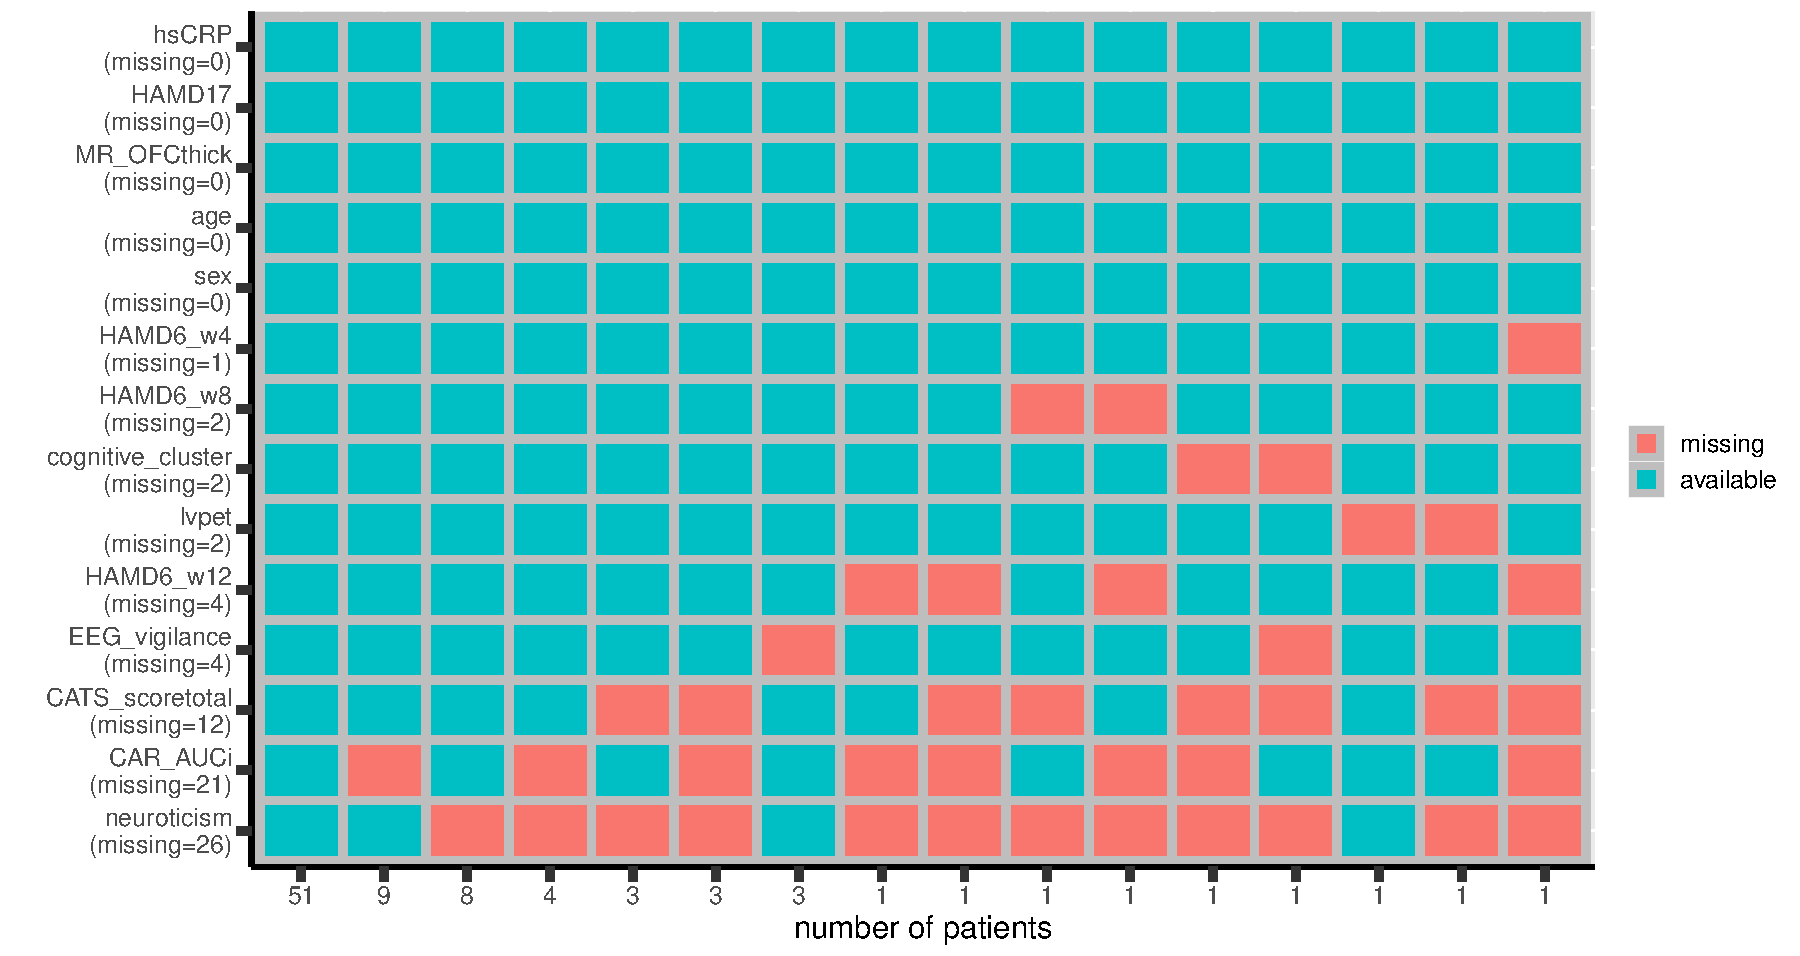
\includegraphics[trim={0 0 0 0},width=0.9\textwidth]{./../figures/gg-missingPattern.pdf}
\caption{\label{fig:missingPattern}Missing data patterns}
\end{figure}

\bigskip
\subsection{Outcome trajectories}
\label{sec:org6231d09}

The following table describes:
\begin{itemize}
\item at week 4: the number of patients that recovered (\texttt{nr2r}) or who did
not recovered (\texttt{nr2nr}).
\item at week 8 and 12: the number of patients who did not recover before
or at the current time (\texttt{nr2nr}), the number of patients who just
recovered (\texttt{nr2r}), the number of patients who recovered previously
but go worse (\texttt{r2nr}), and the number of patients recovered
previously and stay recovered (\texttt{r2r}). \texttt{nr2r+r2r} is then number of
patients currently classified as recovered and \texttt{nr2nr+r2nr} as not
recovered.
\end{itemize}
\phantomsection
\label{}
\begin{verbatim}
            week4        4->8       week8       8->12      week12
nr2nr 52 (58.43%) 30 (34.48%) 40 (45.45%) 20 (23.53%) 26 (30.23%)
r2nr       0 (0%)  9 (10.34%)      0 (0%)   6 (7.06%)      0 (0%)
nr2r  37 (41.57%) 20 (22.99%) 48 (54.55%)    17 (20%) 60 (69.77%)
r2r        0 (0%) 28 (32.18%)      0 (0%) 42 (49.41%)      0 (0%)
total   89 (100%)   87 (100%)   88 (100%)   85 (100%)   86 (100%)
\end{verbatim}


To further describe the outcome trajectory of the patients over time,
we use a latent class linear mixed model with homogeneous residual
variance-covariance between groups to identify 3 groups of
recovery. The results are shown in figure \autoref{fig:hlme} and
ressemble those of \cite{goerigk2021distinct}.

\begin{figure}[!h]
\centering
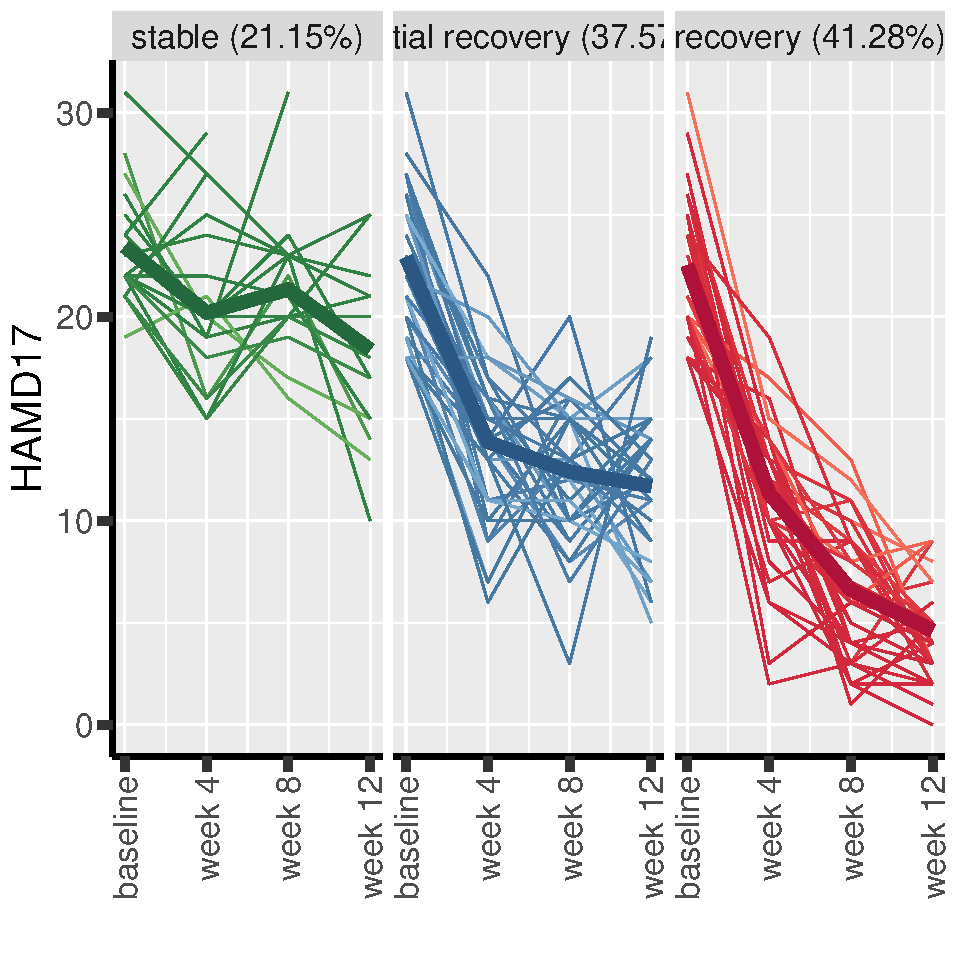
\includegraphics[trim={0 0 0 0},width=0.9\textwidth]{./../figures/spaghetti-HAMD17.pdf}
\caption{\label{fig:hlme}Recovery groups found by a latent class linear mixed model (LCMM). Thin lines represent individual trajectories colored as a function of the group membership probability. Thick lines represent group trajctories estimated by the LCMM.}
\end{figure}
\subsection{Association study (linear)}
\label{sec:orgaf55d8c}

The following table shows the result of multiple imputation for the
logistic model with biomarkers at week 8, based on 88 patients (some
with missing biomarker values):
\phantomsection
\label{}
\begin{verbatim}
                     term estimate std.error p.value adj.p.value lower.adj upper.adj
 1:                female -0.57753    0.5927 0.33311          NA        NA        NA
 2:                   age  0.45193    0.3248 0.16839          NA        NA        NA
 3:       PET (serotonin) -0.09617    0.2602 0.71280     0.99999   -0.8433    0.6510
 4:    MR (OFC thickness) -0.48612    0.2888 0.09664     0.59434   -1.3153    0.3431
 5:       EEG (vigilance) -0.69847    0.2940 0.02015     0.17150   -1.5426    0.1456
 6:                 hsCRP  0.89400    0.6496 0.17305     0.81272   -0.9709    2.7589
 7:              Cortisol  0.28153    0.2963 0.34521     0.97702   -0.5691    1.1322
 8: cognition (cluster 2) -0.69912    0.6319 0.27222     0.93997   -2.5132    1.1150
 9: cognition (cluster 3) -1.87992    0.7110 0.01004     0.09045   -3.9210    0.1612
10:                HAMD17  0.32098    0.2704 0.23911     0.91059   -0.4554    1.0974
11:           Neuroticism  0.22613    0.3346 0.50133     0.99819   -0.7346    1.1868
12:                  CATS  0.07479    0.2752 0.78656     1.00000   -0.7153    0.8648
\end{verbatim}

The smallest adjusted p-value is 0.09 obtained for cognition cluster
3: being is this cluser is associated with lower remission rate
(estimate OR=exp(-1.8799)=0.153). The second most significant p-value
is obtained for EEG (estimate OR=exp(-0.698)=0.497).

\clearpage

\textbf{Sensitivity analysis}: we replicated this analysis at week 4:
\phantomsection
\label{}
\begin{verbatim}
                     term estimate std.error p.value adj.p.value lower.adj upper.adj
 1:                female -1.15006    0.5764 0.04969          NA        NA        NA
 2:                   age  0.24250    0.2627 0.35894          NA        NA        NA
 3:       PET (serotonin)  0.08062    0.2491 0.74716      1.0000   -0.6350    0.7962
 4:    MR (OFC thickness) -0.05876    0.2573 0.81995      1.0000   -0.7978    0.6803
 5:       EEG (vigilance) -0.10138    0.2506 0.68696      1.0000   -0.8212    0.6184
 6:                 hsCRP  0.65041    0.6535 0.32293      0.9707   -1.2268    2.5277
 7:              Cortisol  0.28874    0.3055 0.34776      0.9793   -0.5889    1.1664
 8: cognition (cluster 2) -0.33296    0.6005 0.58099      0.9997   -2.0581    1.3921
 9: cognition (cluster 3) -1.30528    0.6729 0.05631      0.4106   -3.2383    0.6278
10:                HAMD17  0.08812    0.2541 0.72970      1.0000   -0.6417    0.8180
11:           Neuroticism  0.20053    0.3165 0.52825      0.9990   -0.7085    1.1096
12:                  CATS -0.28135    0.2800 0.31831      0.9689   -1.0858    0.5231
\end{verbatim}

and week 12:
\phantomsection
\label{}
\begin{verbatim}
                     term estimate p.value adj.p.value lower.adj upper.adj
 1:                female -0.91744 0.18901          NA        NA        NA
 2:                   age  0.73698 0.13716          NA        NA        NA
 3:       PET (serotonin)  0.14969 0.61394     0.99982   -0.6977   0.99712
 4:    MR (OFC thickness) -0.87021 0.01060     0.09396   -1.8210   0.08061
 5:       EEG (vigilance) -0.05549 0.85470     1.00000   -0.9215   0.81049
 6:                 hsCRP  0.54170 0.48043     0.99699   -1.6487   2.73211
 7:              Cortisol  0.46282 0.22519     0.88904   -0.6222   1.54790
 8: cognition (cluster 2) -1.23228 0.11663     0.65759   -3.4573   0.99276
 9: cognition (cluster 3) -1.23212 0.14918     0.75138   -3.6555   1.19129
10:                HAMD17  0.22865 0.43895     0.99386   -0.6140   1.07128
11:           Neuroticism -0.02338 0.95341     1.00000   -1.1672   1.12048
12:                  CATS  0.69398 0.04752     0.34997   -0.2932   1.68113
\end{verbatim}

At week 4 we see again some evidence for cluster 3 (without adjustment
for multiple comparisons). At week 12, the most promising biomarkers
would be OFC thickness and CATS.

\clearpage

We also replicated the analysis when removing CATS, Cortisol,
Neuroticm and using a complete case approach. The results are
summarized on the following forest plot (\autoref{fig:forestPlot}) and in the table below for week 8:
\phantomsection
\label{}
\begin{verbatim}
                     term estimate std.error p.value adj.p.value lower.adj upper.adj
 1:                   age   0.4608    0.3319 0.16502          NA        NA        NA
 2:                female  -0.4576    0.5955 0.44219          NA        NA        NA
 3:       PET (serotonin)  -0.1501    0.2587 0.56169      0.9961   -0.8421    0.5419
 4:    MR (OFC thickness)  -0.4546    0.2971 0.12598      0.5899   -1.2493    0.3402
 5:       EEG (vigilance)  -0.6594    0.2933 0.02455      0.1544   -1.4440    0.1252
 6:                 hsCRP   0.8238    0.6364 0.19551      0.7626   -0.8788    2.5264
 7:              Cortisol       NA        NA      NA          NA        NA        NA
 8: cognition (cluster 2)  -0.5081    0.6222 0.41419      0.9716   -2.1727    1.1566
 9: cognition (cluster 3)  -1.3911    0.6773 0.03999      0.2394   -3.2031    0.4210
10:                HAMD17   0.2816    0.2897 0.33118      0.9306   -0.4936    1.0568
11:           Neuroticism       NA        NA      NA          NA        NA        NA
12:                  CATS       NA        NA      NA          NA        NA        NA
\end{verbatim}

We note that for some variables (age, cognition cluster 2, OFC
thickness) the association seemed more and more pronounced over the
weeks. The odds ratio for cognition cluster 3 and EEG vigilance are
0.249 and 0.517, respectively.

\begin{figure}[!h]
\centering
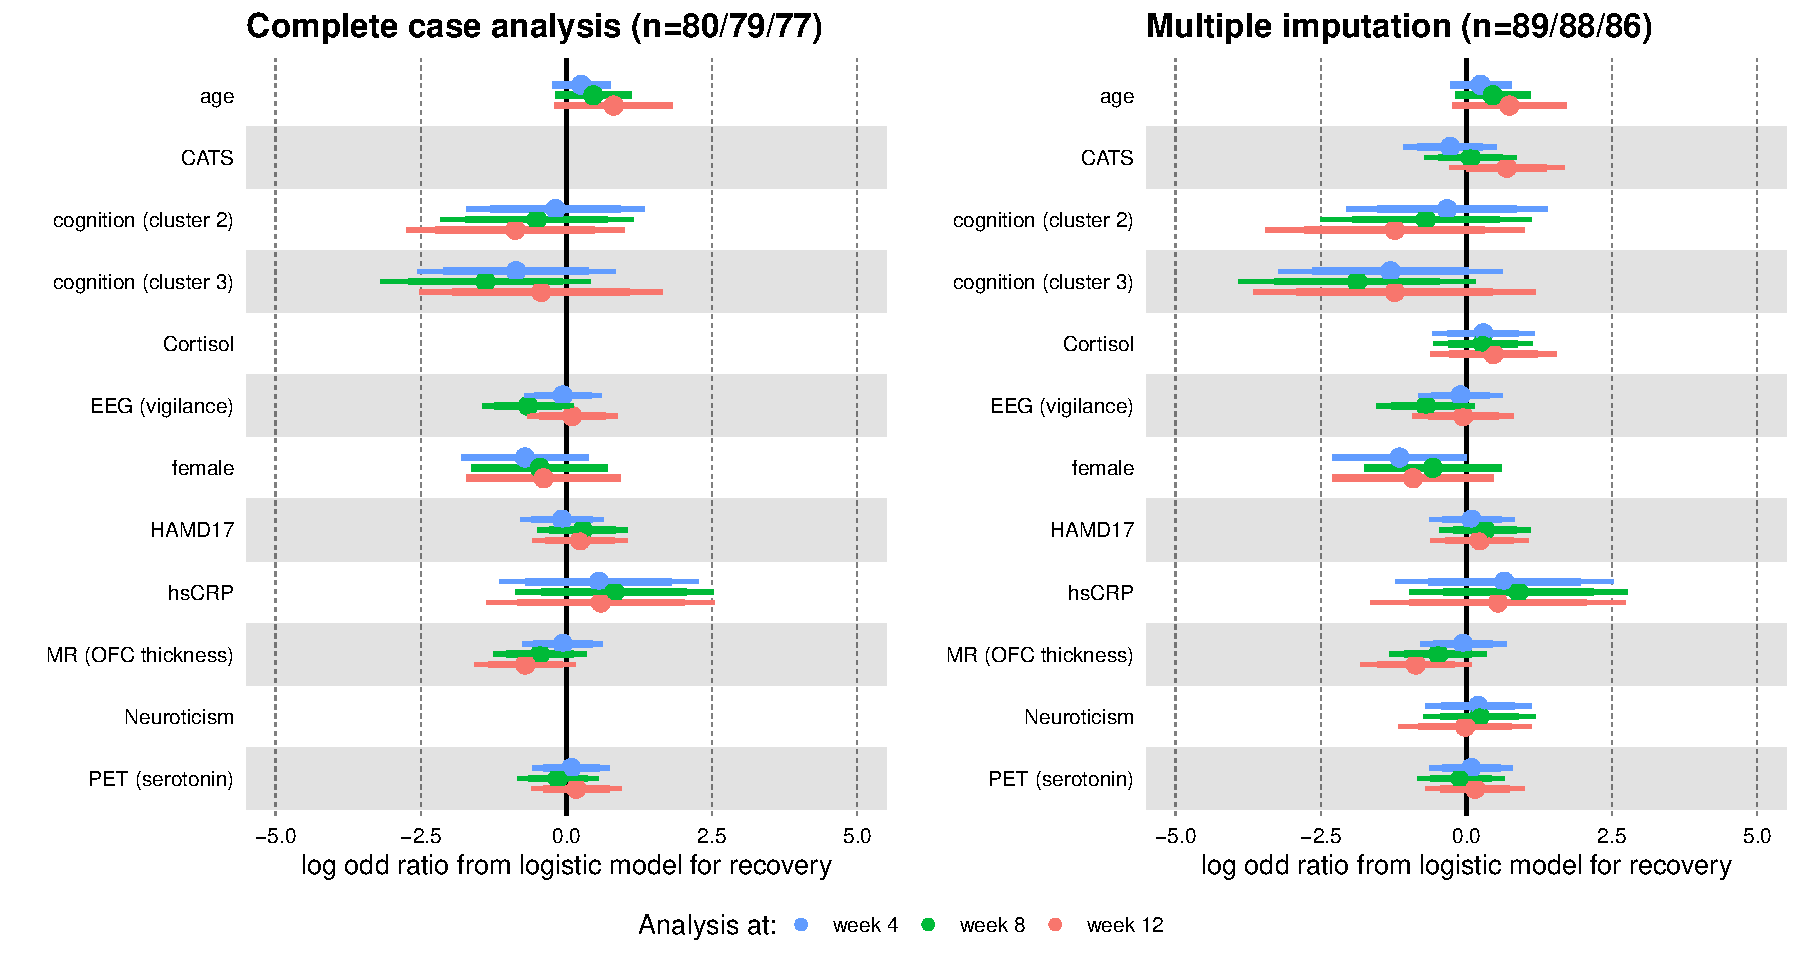
\includegraphics[trim={0 0 0 0},width=\textwidth]{./../figures/gg-forestplot-OR.pdf}
\caption{\label{fig:forestPlot}Log-odd ratio estimates (full circles), confidence intervals (thick lines) and adjusted confidence intervals (thin lines) for each analysis at each timepoint. Covariates have been centered and scale to be comparable. Adjustment for multiplicity is performed over biomarkers but not over time.}
\end{figure}
\subsection{Association study (non-linear)}
\label{sec:orgdb58d78}

When using random forest with the complete case approach, no biomarker
appeared relevant at week 8 (see also \autoref{fig:variableImportance}):
\phantomsection
\label{}
\begin{verbatim}
                  param              week4              week8             week12
1                female -0.0051 (p=0.8771) -0.0052 (p=0.8741) -0.0035 (p=0.7722)
2                   age  0.0146 (p=0.1329)  0.0117 (p=0.1439) -0.0012 (p=0.5165)
3    MR (OFC thickness)   0.005 (p=0.3117)  0.0077 (p=0.2597)  0.0163 (p=0.0899)
4                HAMD17 -0.0107 (p=0.8841)  0.0055 (p=0.2567)   6e-04 (p=0.4356)
5                 hsCRP -0.0018 (p=0.5804) -0.0043 (p=0.8392) -0.0032 (p=0.8302)
6       PET (serotonin)  0.0043 (p=0.3207) -0.0103 (p=0.7792)    0.022 (p=0.037)
7 cognition (cluster 2) -0.0011 (p=0.5015)  -5e-04 (p=0.4426)  0.0029 (p=0.2118)
8 cognition (cluster 3)  0.0075 (p=0.0789)   0.0098 (p=0.039)  -8e-04 (p=0.4985)
9       EEG (vigilance) -0.0039 (p=0.7103)  0.0055 (p=0.1888)  0.0042 (p=0.2108)
\end{verbatim}

At week 4 and 8, cognition (cluster) 3 was borderline significant. At
week 12, there was some evidence for PET, and to a lesser extend for
OFC thickness, to be associated with the recovery.

\begin{figure}[!h]
\centering
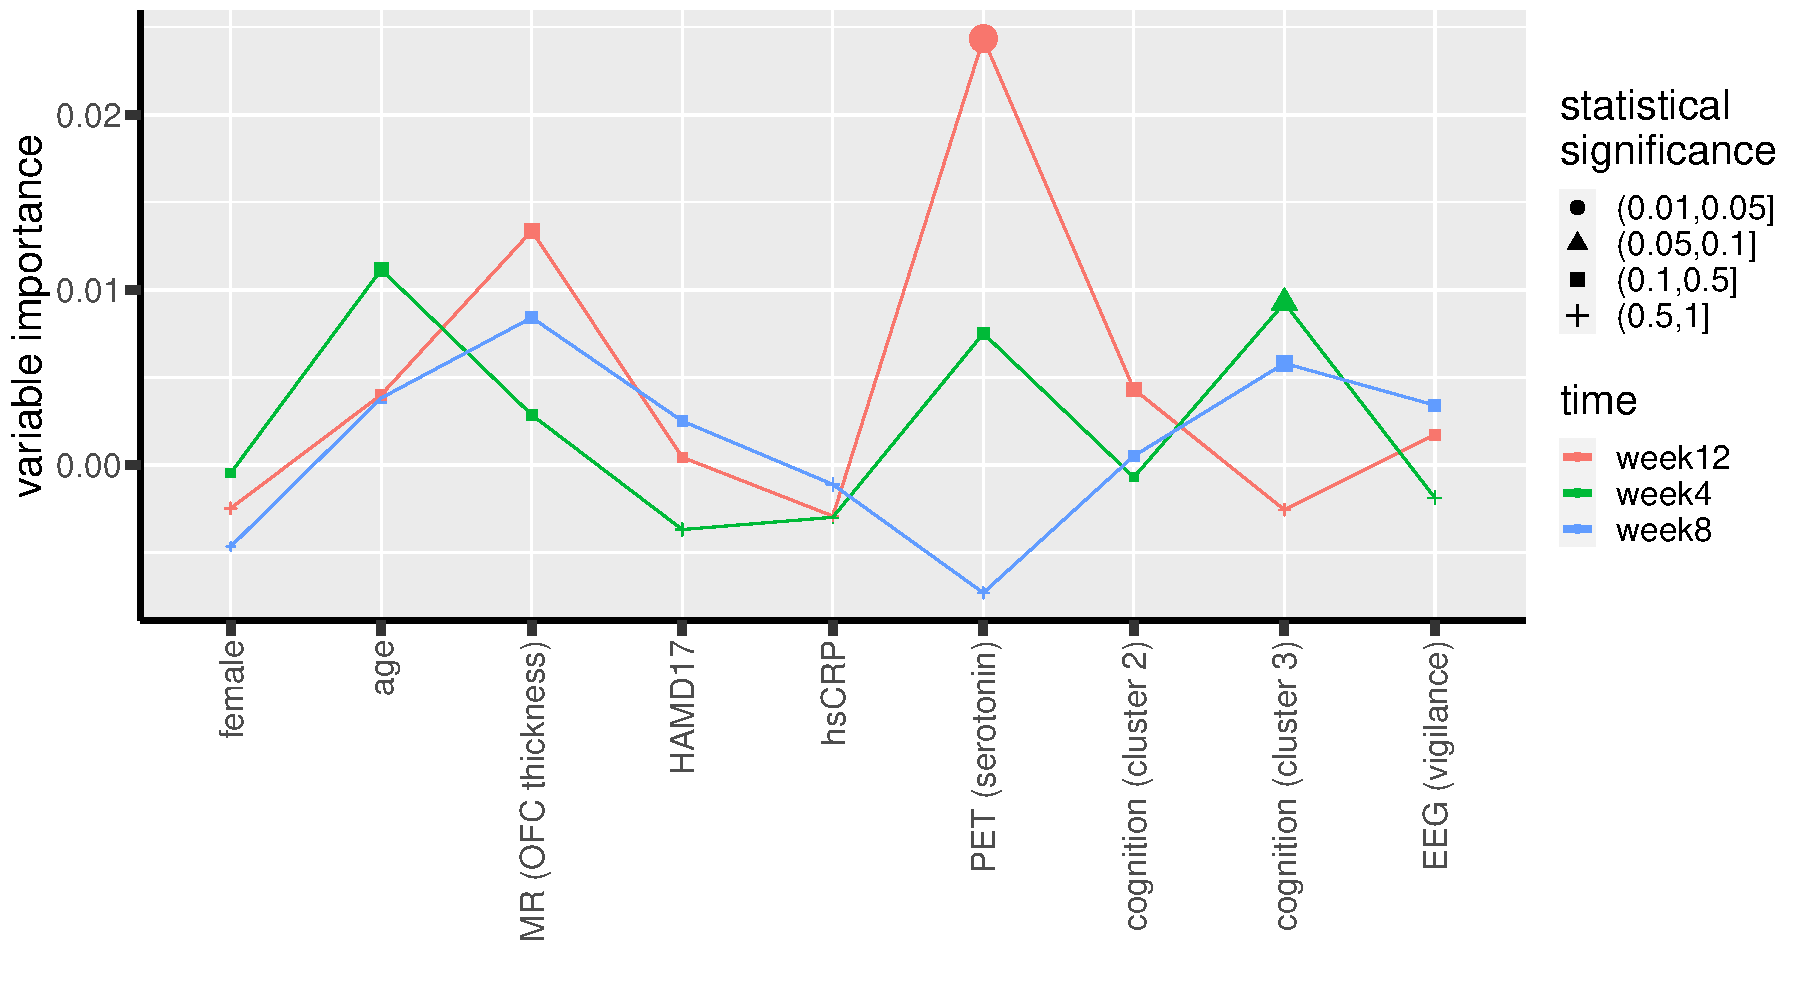
\includegraphics[trim={0 0 0 0},width=\textwidth]{./../figures/variableImportance.pdf}
\caption{\label{fig:variableImportance}Variable importance (y-axis) and associated statistical significance (size of the point) of the predictors in a random forest model (complete case analysis).}
\end{figure}

\clearpage

Further investigation using splines reveal an inverted U-shape for the
PET assocation (\autoref{fig:splineW12}, p=0.022). A similar but non
significant association was observed for PET at week 8 (\autoref{fig:splineW8},
p=0.0904).
\vfill

\begin{figure}[!h]
\centering
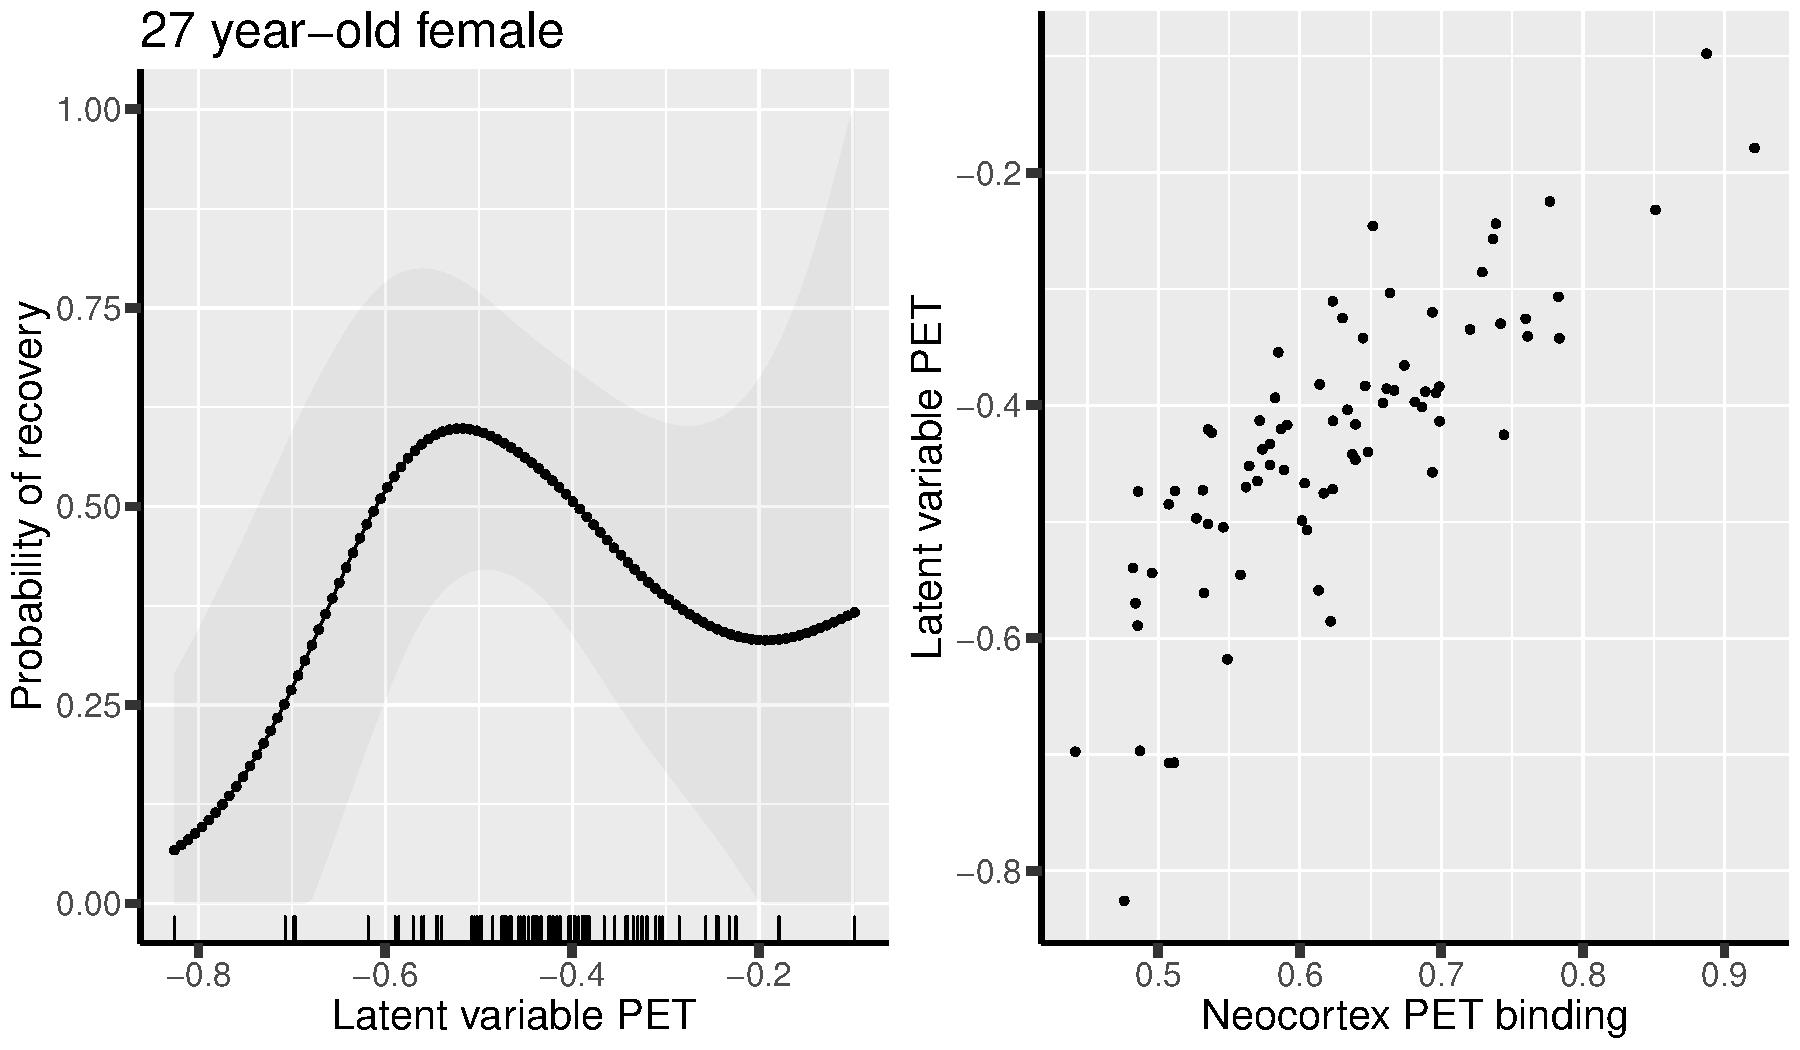
\includegraphics[trim={0 0 0 0},width=0.8\textwidth]{./../figures/gg-spline-w8.pdf}
\caption{\label{fig:splineW8}Association between recovery at week 8 and PET in a logistic model adjusted for age and sex (complete case).}
\end{figure}

\begin{figure}[!h]
\centering
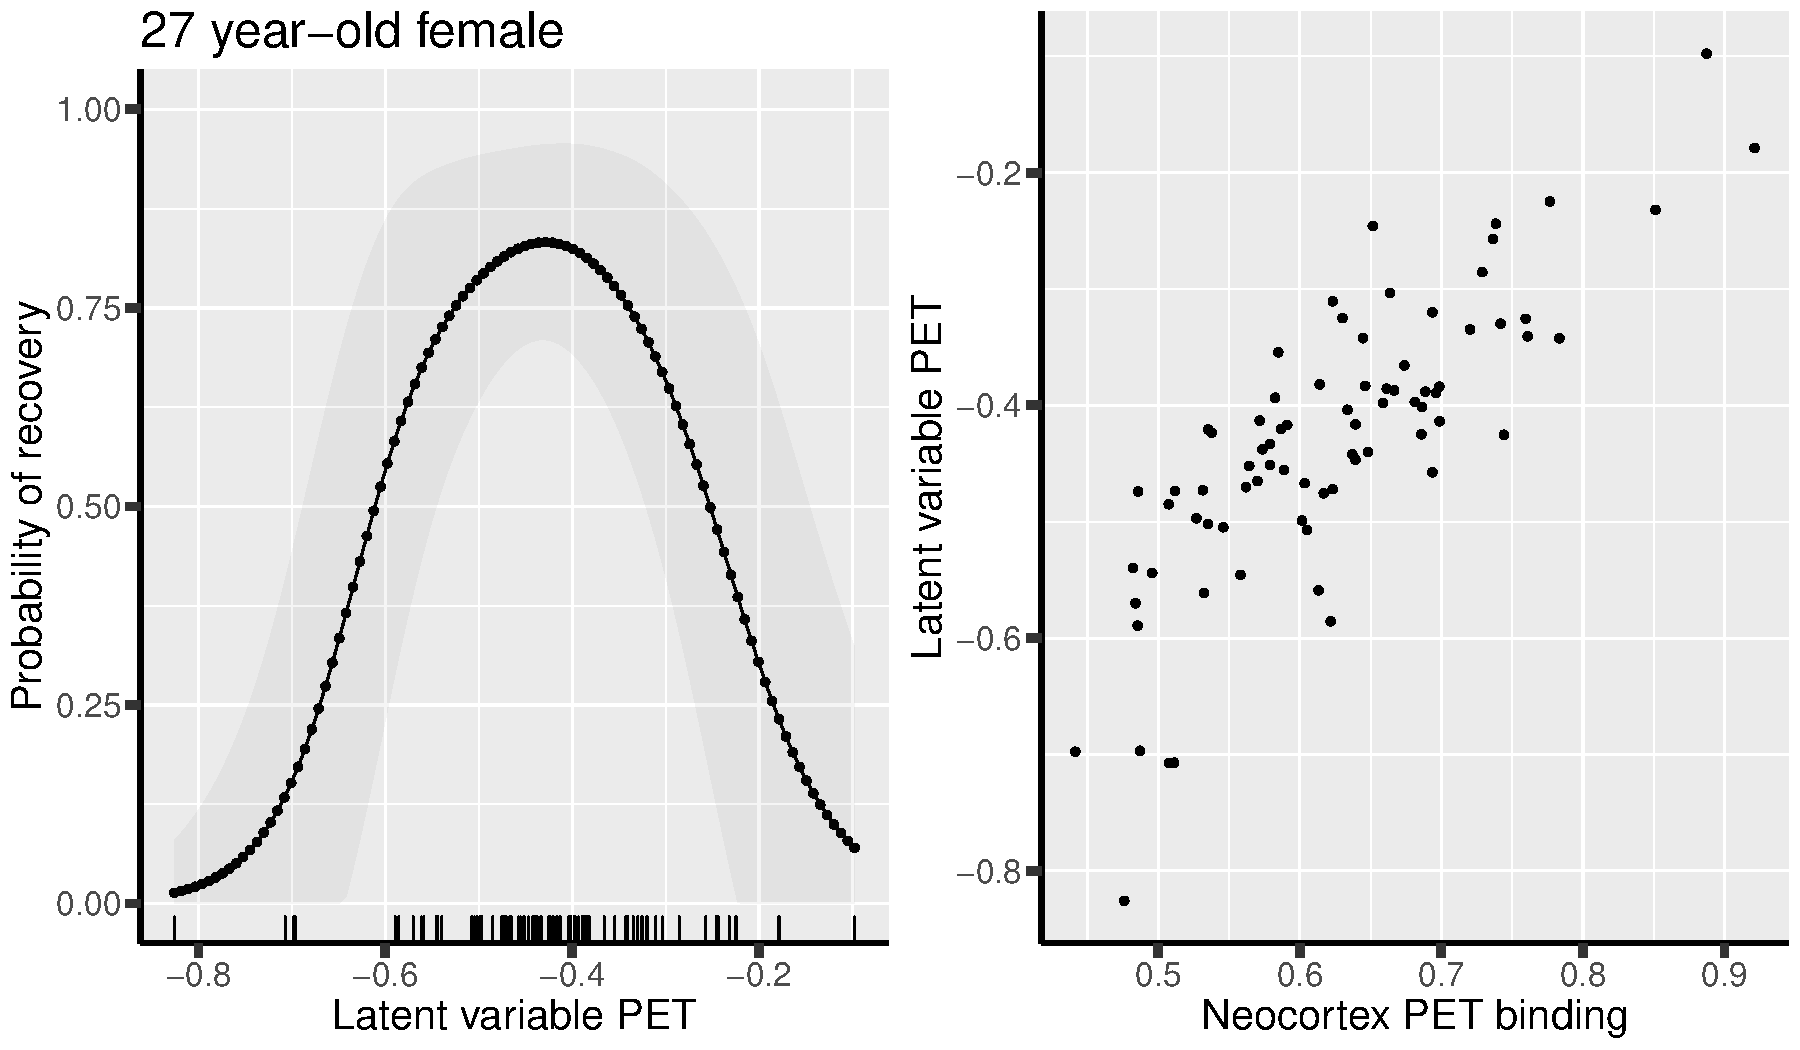
\includegraphics[trim={0 0 0 0},width=0.8\textwidth]{./../figures/gg-spline-w12.pdf}
\caption{\label{fig:splineW12}Association between recovery at week 12 and PET in a logistic model adjusted for age and sex (complete case).}
\end{figure}

\clearpage
\subsection{Predictive value}
\label{sec:org6e03bf3}

\autoref{fig:perfW4-dens}, \autoref{fig:perfW8-dens}, and
\autoref{fig:perfW12-dens} display the predicted probability obtain
after cross-validation colored by recovery group. Overall it looks
that the group are comparable at week 4 but there may be a difference
at week 8 and 12. The corresponding ROC curve are put in appendix
(\autoref{fig:perfW4-ROC}, \autoref{fig:perfW8-ROC},
\autoref{fig:perfW12-ROC}).

\begin{figure}[!h]
\centering
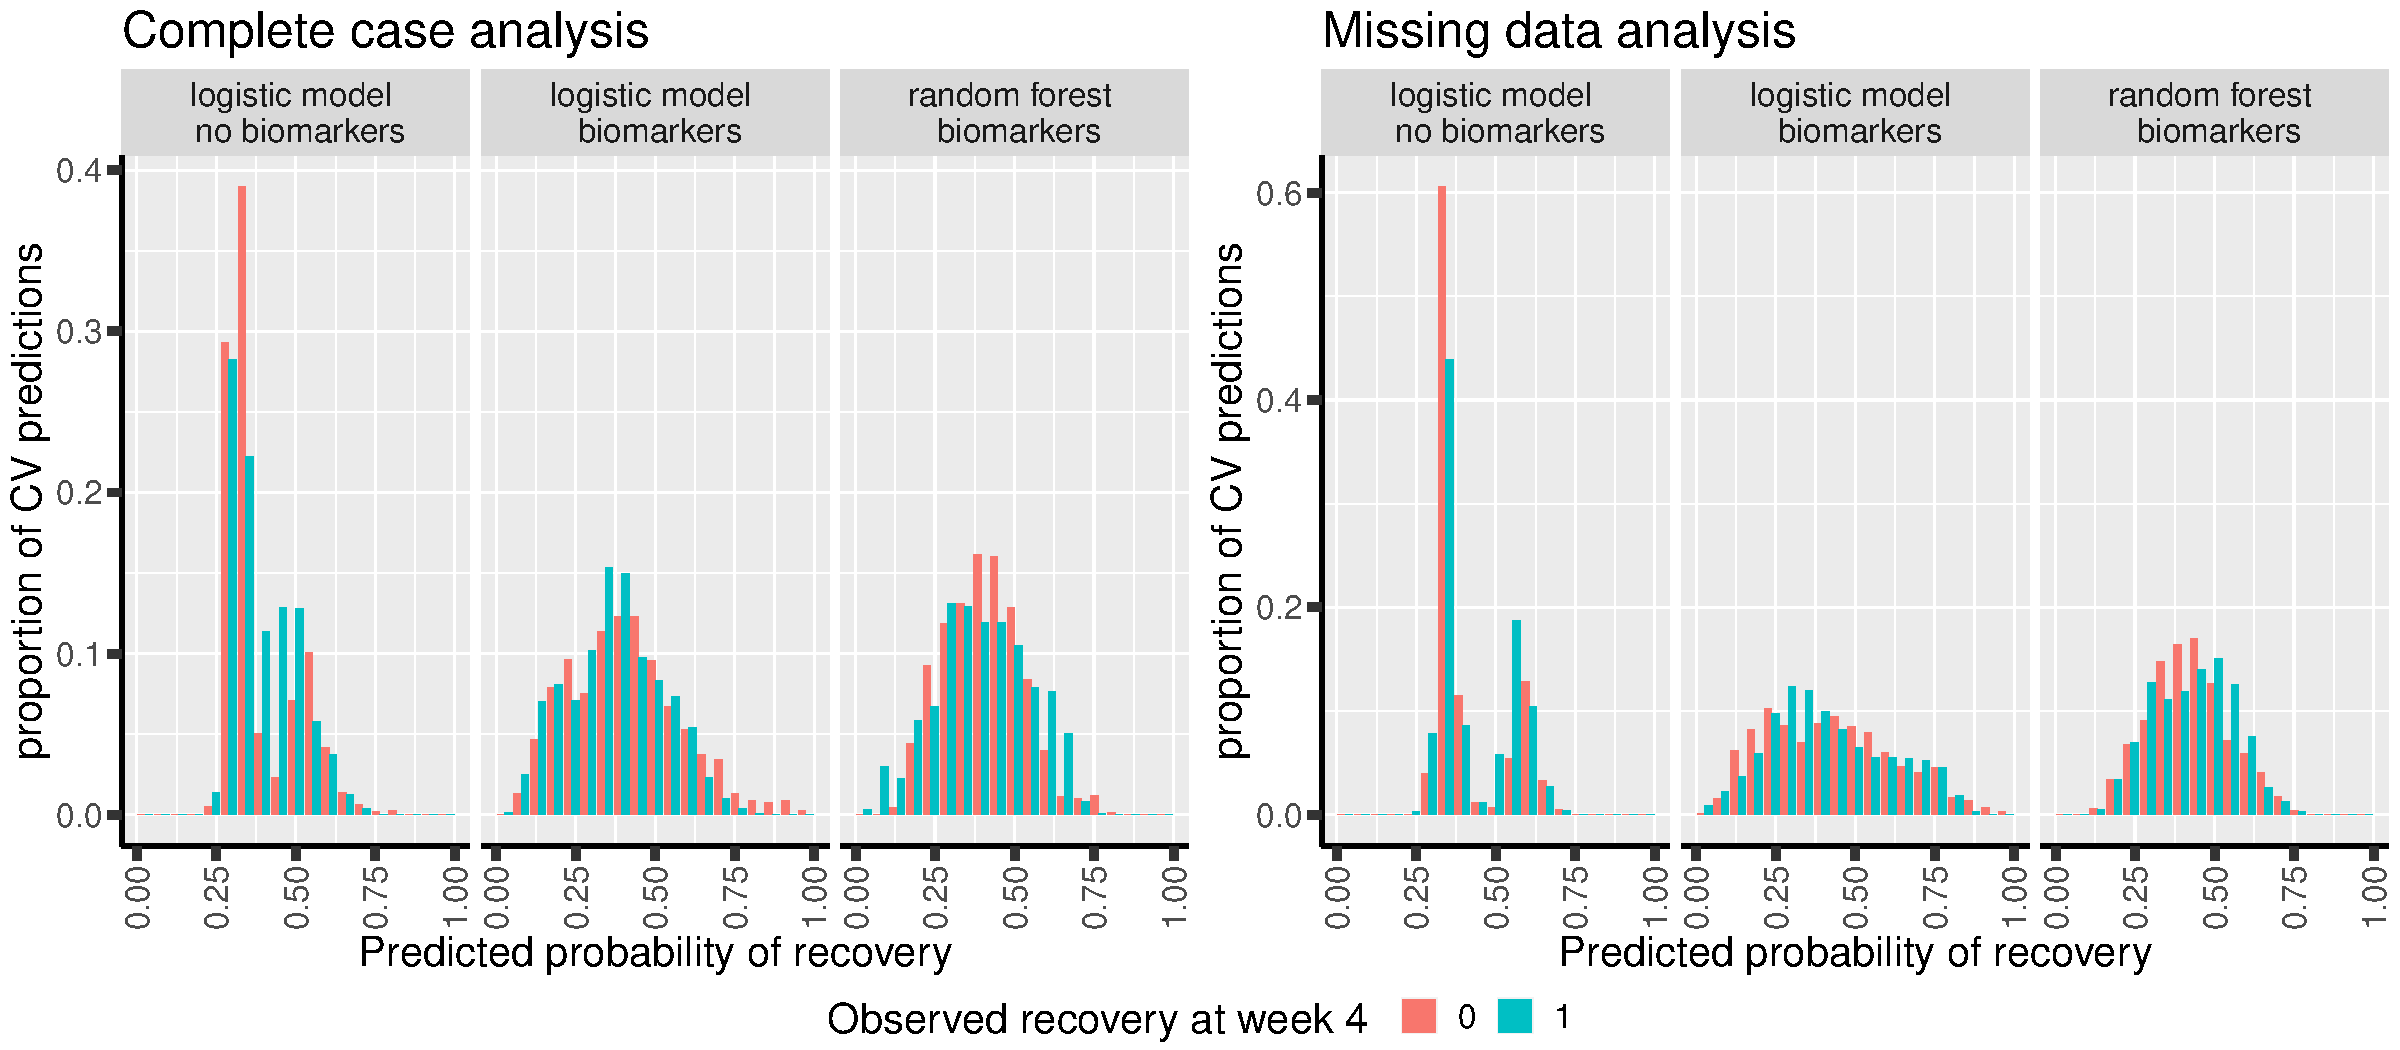
\includegraphics[trim={0 0 0 0},width=\textwidth]{./../figures/hist-pred-week4.pdf}
\caption{\label{fig:perfW4-dens}Distribution of the predicted probability of recovery at week 4 per group according to each model.}
\end{figure}

\begin{figure}[!h]
\centering
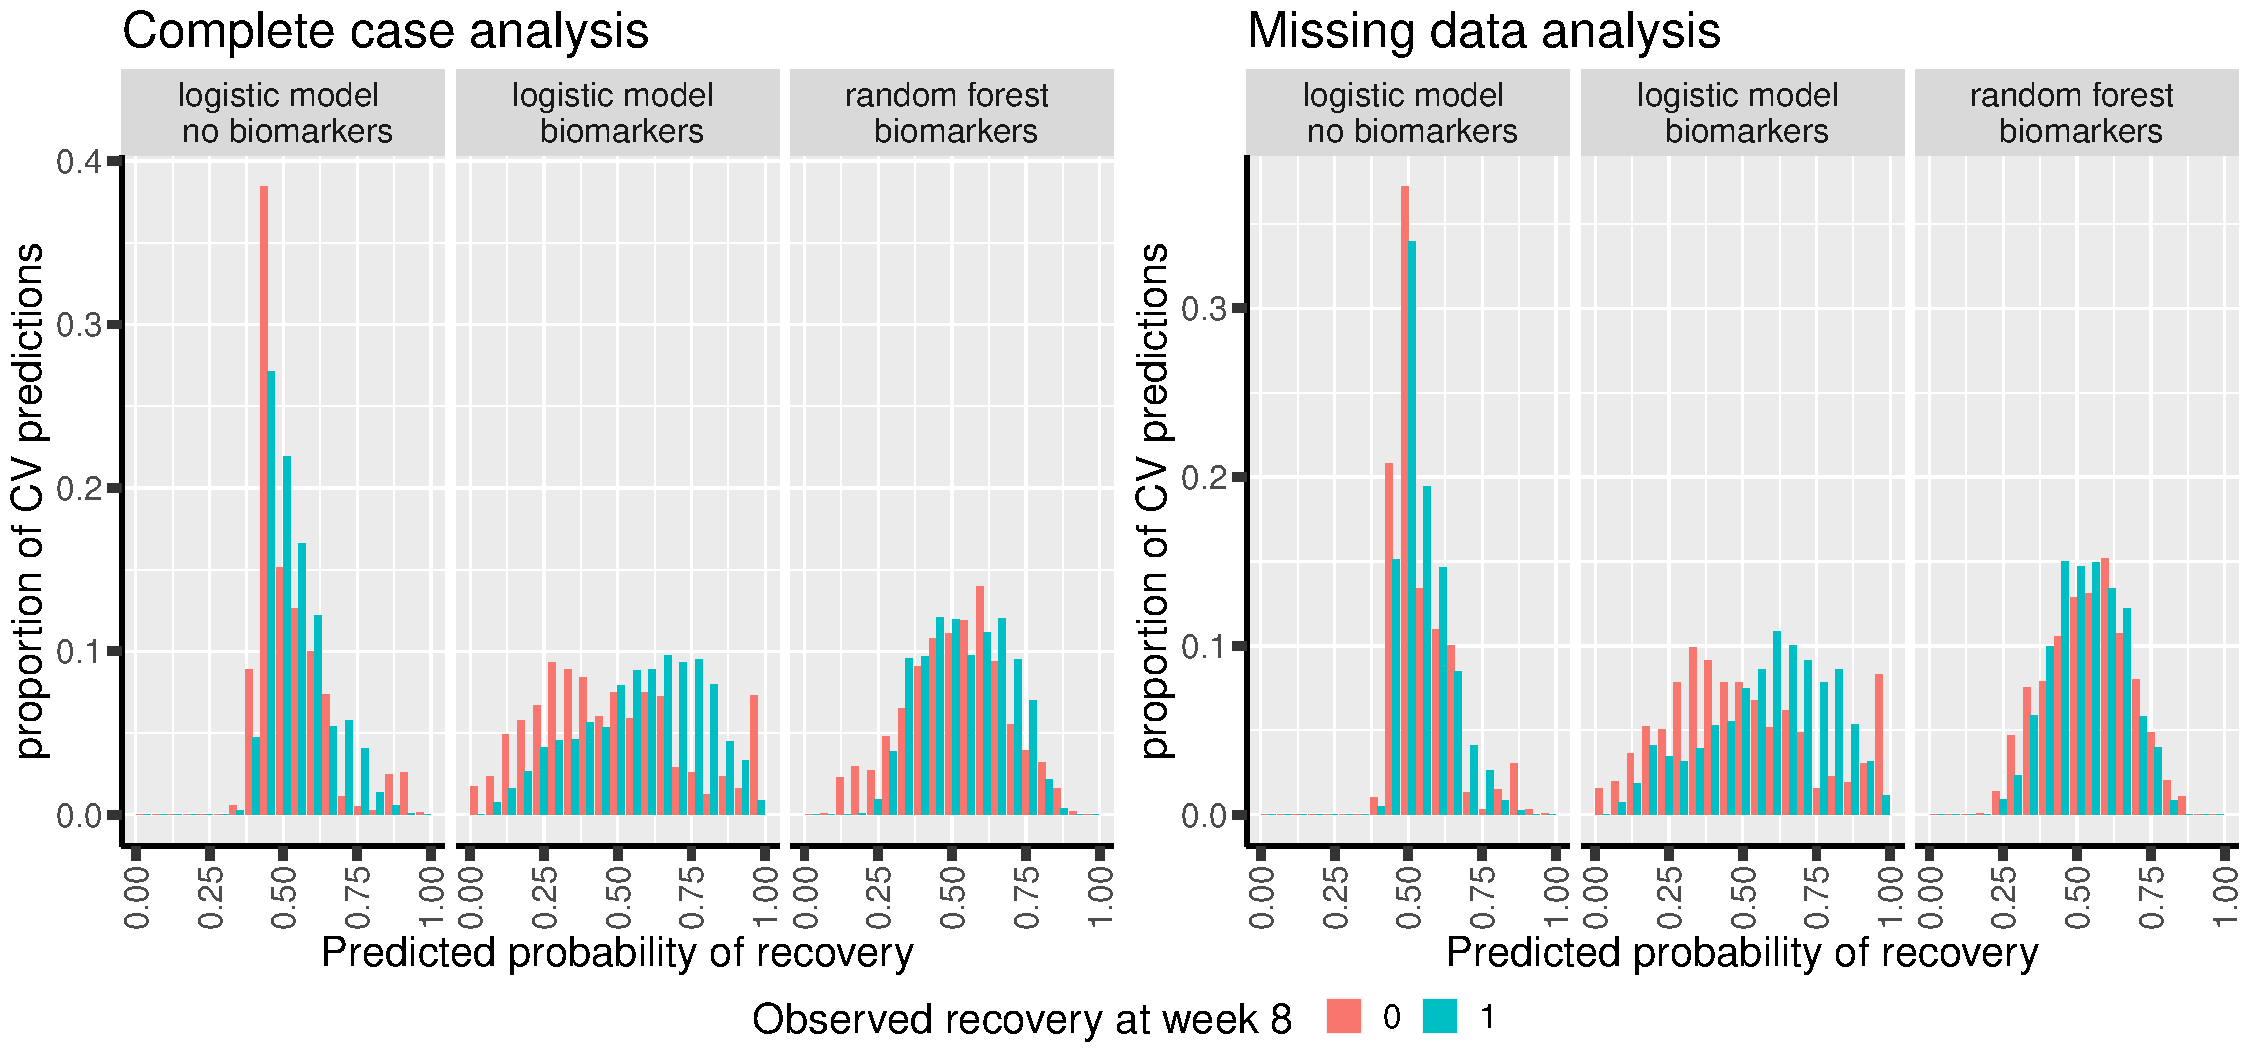
\includegraphics[trim={0 0 0 0},width=\textwidth]{./../figures/hist-pred-week8.pdf}
\caption{\label{fig:perfW8-dens}Distribution of the predicted probability of recovery at week 8 per group according to each model.}
\end{figure}

\clearpage

\begin{figure}[!h]
\centering
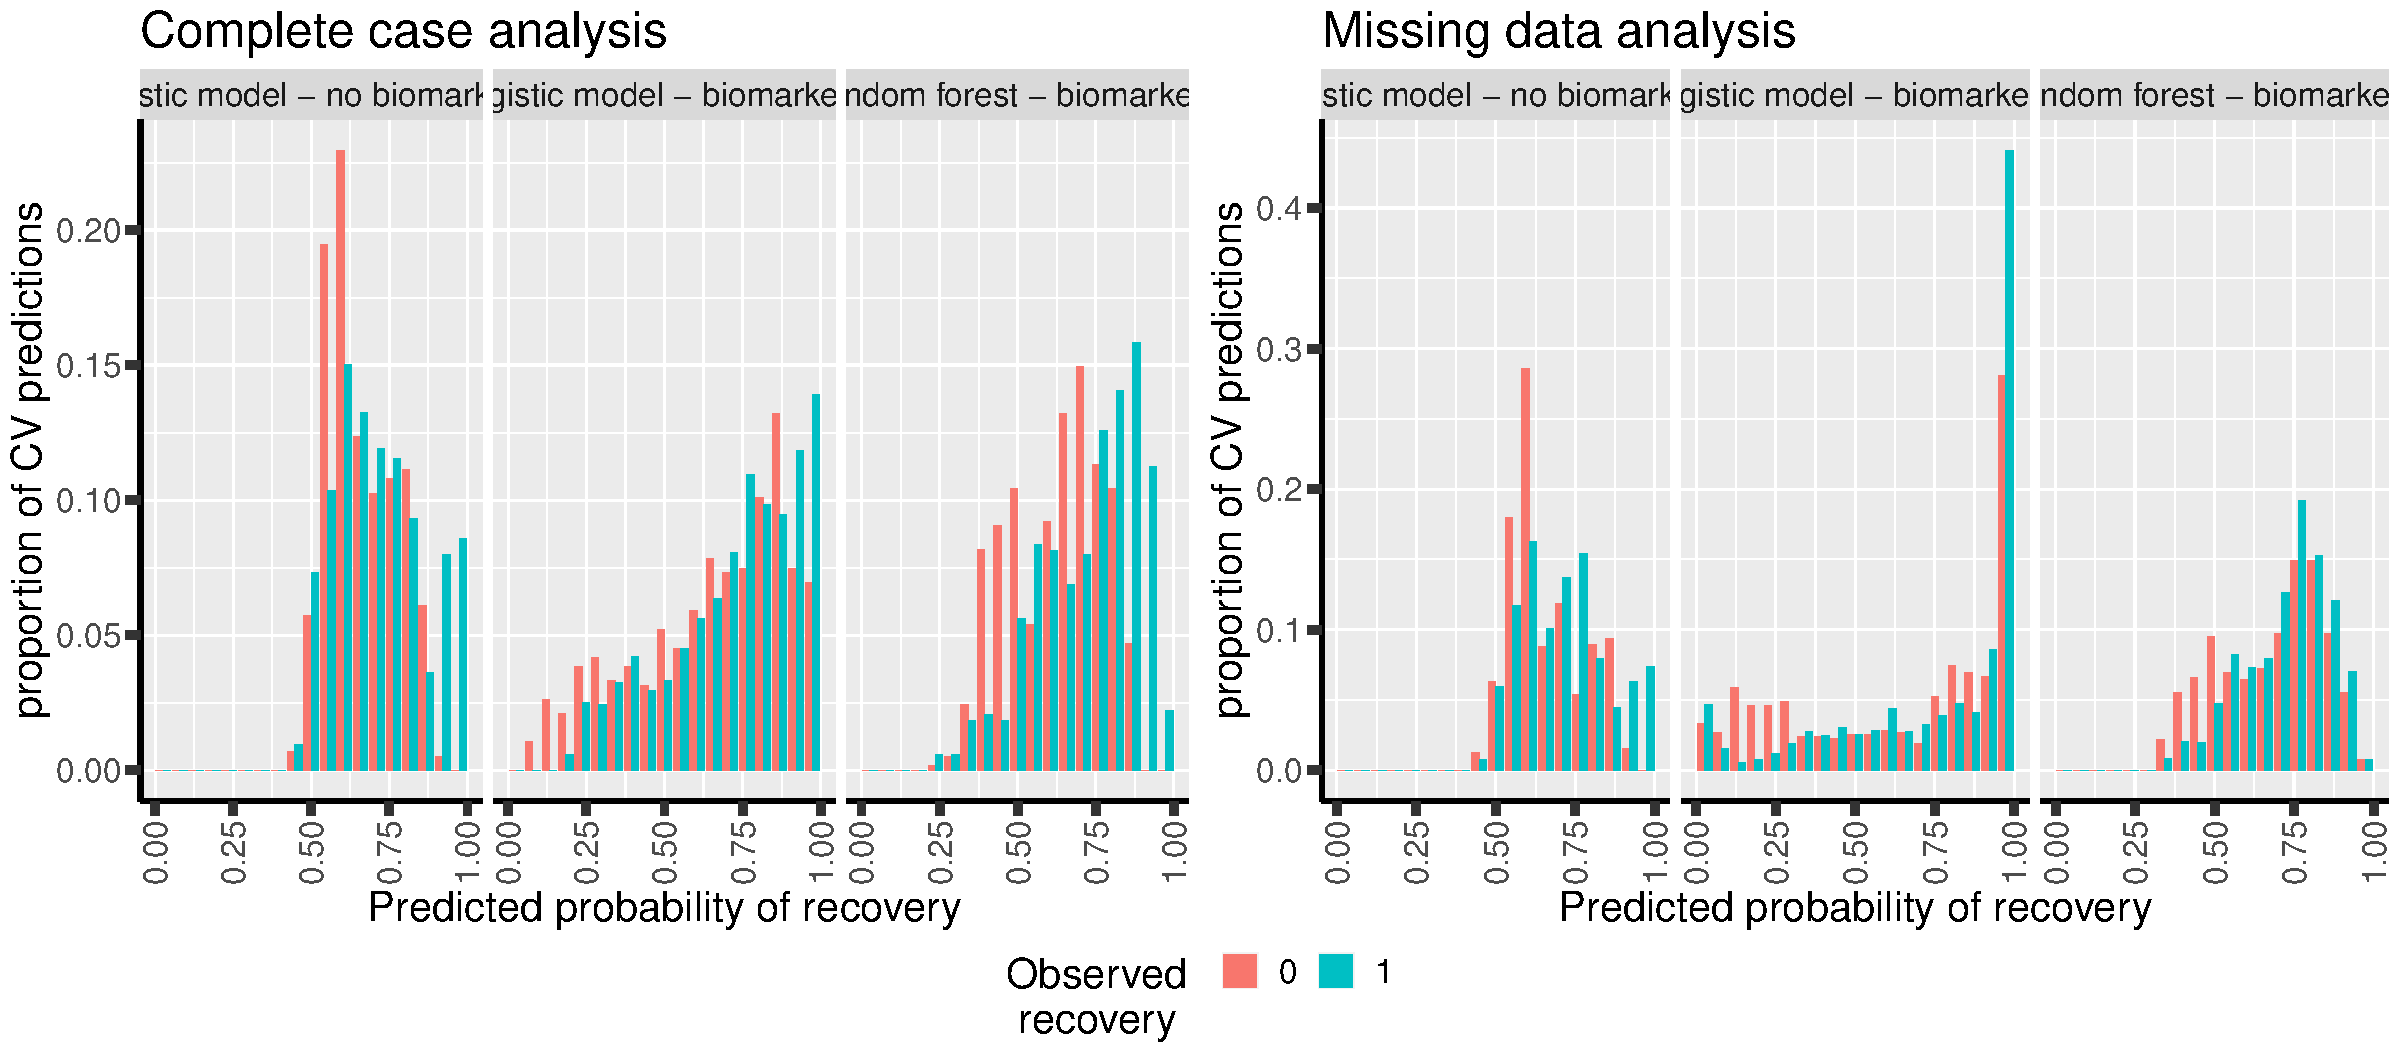
\includegraphics[trim={0 0 0 0},width=\textwidth]{./../figures/hist-pred-week12.pdf}
\caption{\label{fig:perfW12-dens}Distribution of the predicted probability of recovery at week 12 per group according to each model.}
\end{figure}

The table below summarizes the predictive performance. There was some
evidence for a discriminative power at week 8 (AUC=0.621, p=0.059) of
the logistic regression with biomarkers. But not enough (p=0.327) to
show superiority compared to a model without biomarkers. Similar
results were observed in term of calibration, i.e. brier score. Random
forest appeared to provide worse predictions at that timepoint.

\bigskip

None of the prediction methods performed well at week 4 while at week
12 all of them were marginally better than chance. Random Forest had
an AUC of 0.635 (p=0.044) which is very similar to the AUC=0.622 of
the model with age and sex alone.

\phantomsection
\label{}
\begin{verbatim}
                model week                                AUC                 Brier
1: GLM (no biomarker)    4 0.514 (p(IF)=0.812, p(perm)=0.272) 0.245 (p(perm)=0.179)
2:                       8 0.549 (p(IF)=0.420, p(perm)=0.152) 0.253 (p(perm)=0.289)
3:                      12 0.622 (p(IF)=0.079, p(perm)=0.031) 0.204 (p(perm)=0.033)
4:   GLM (biomarkers)    4 0.489 (p(IF)=0.847, p(perm)=0.521) 0.287 (p(perm)=0.471)
5:                       8 0.621 (p(IF)=0.059, p(perm)=0.068) 0.258 (p(perm)=0.057)
6:                      12 0.617 (p(IF)=0.098, p(perm)=0.072) 0.227 (p(perm)=0.061)
7:    RF (biomarkers)    4  0.52 (p(IF)=0.739, p(perm)=0.390) 0.256 (p(perm)=0.399)
8:                       8 0.478 (p(IF)=0.710, p(perm)=0.596) 0.269 (p(perm)=0.615)
9:                      12 0.635 (p(IF)=0.044, p(perm)=0.044) 0.203 (p(perm)=0.050)
\end{verbatim}

\clearpage

\bigskip

\textbf{Sensitivity analysis}: Similar results were obtained with the
complete case analysis (which also drop 3 biomarkers):
\phantomsection
\label{}
\begin{verbatim}
                 model       week                                 AUC                 Brier
 1: GLM (no biomarker)          4 0.529 (p(IF)=0.6592, p(perm)=0.215) 0.244 (p(perm)=0.328)
 2:                             8 0.582 (p(IF)=0.2119, p(perm)=0.073) 0.253 (p(perm)=0.206)
 3:                            12 0.615 (p(IF)=0.1089, p(perm)=0.033) 0.204 (p(perm)=0.037)
 4:                    trajectory 0.604 (p(IF)=0.1241, p(perm)=0.043)  0.23 (p(perm)=0.030)
 5:   GLM (biomarkers)          4 0.443 (p(IF)=0.3290, p(perm)=0.733) 0.285 (p(perm)=0.787)
 6:                             8 0.644 (p(IF)=0.0338, p(perm)=0.034)  0.25 (p(perm)=0.031)
 7:                            12 0.583 (p(IF)=0.2447, p(perm)=0.149)  0.23 (p(perm)=0.156)
 8:                    trajectory 0.645 (p(IF)=0.0341, p(perm)=0.026) 0.244 (p(perm)=0.035)
 9:    RF (biomarkers)          4  0.49 (p(IF)=0.8708, p(perm)=0.536)  0.26 (p(perm)=0.549)
10:                             8  0.54 (p(IF)=0.5256, p(perm)=0.306)  0.26 (p(perm)=0.286)
11:                            12 0.694 (p(IF)=0.0046, p(perm)=0.013) 0.193 (p(perm)=0.020)
12:                    trajectory 0.597 (p(IF)=0.1321, p(perm)=0.104) 0.238 (p(perm)=0.103)
\end{verbatim}

The main difference being at week 12 where the RF results appeared
better (both in term of AUC and brier score) and the logistic model
worse.

\clearpage
\section{Conclusion}
\label{sec:org529cacc}

There is some evidence that cognition and EEG (and to a lesser extend
OFC thickness) are predictive of recovery at week 8. By some evidence,
we mean that the unadjusted p-value was significant (between 0.01 and
0.05) while the adjusted p-value was above the traditional threshold
(typically around 0.1). There was also some evidence for a predictive
value of these biomarkers: performance superior to the null predictor
and pointwise estimate of the in gain in AUC when adding the
biomarkers of about +0.11. So while the biomarkers may help to
discriminate between patients who will recover or not, it seems that
we are not able to obtain reliable (nor clinically relevant)
probabilities of recovery. \newline Using a flexible model such as
random forest did not seems to help, which is to be expected with a
rather limited sample size.

\bigskip

Time at which recovery was assessed also appeared to have a impact on
 the results. For instance the value of EEG was only evident at
 week 8. Cognition seemed to have a more stable association with
 recovery while others like age or OFC thickness the strength of
 assocation seemed to increase over time. Overall, there was no
 evidence that the biomarkers were useful at week 4 while there was
 some evidence at week 12, probably due to <due to OFC thickness and
 PET.
\section{References}
\label{sec:org090f06c}
\begingroup
\renewcommand{\section}[2]{}
\bibliographystyle{apalike}
\bibliography{bibliography}

\endgroup

\appendix
\titleformat{\section}
{\normalfont\Large\bfseries}{Appendix~\thesection}{1em}{}

\renewcommand{\thefigure}{\Alph{figure}}
\renewcommand{\thetable}{\Alph{table}}
\renewcommand{\theequation}{\Alph{equation}}

\setcounter{figure}{0}    
\setcounter{table}{0}    
\setcounter{equation}{0}    

\setcounter{page}{1}

\clearpage
\section{ROC curves}
\label{appendix:ROC}
\begin{figure}[!h]
\centering
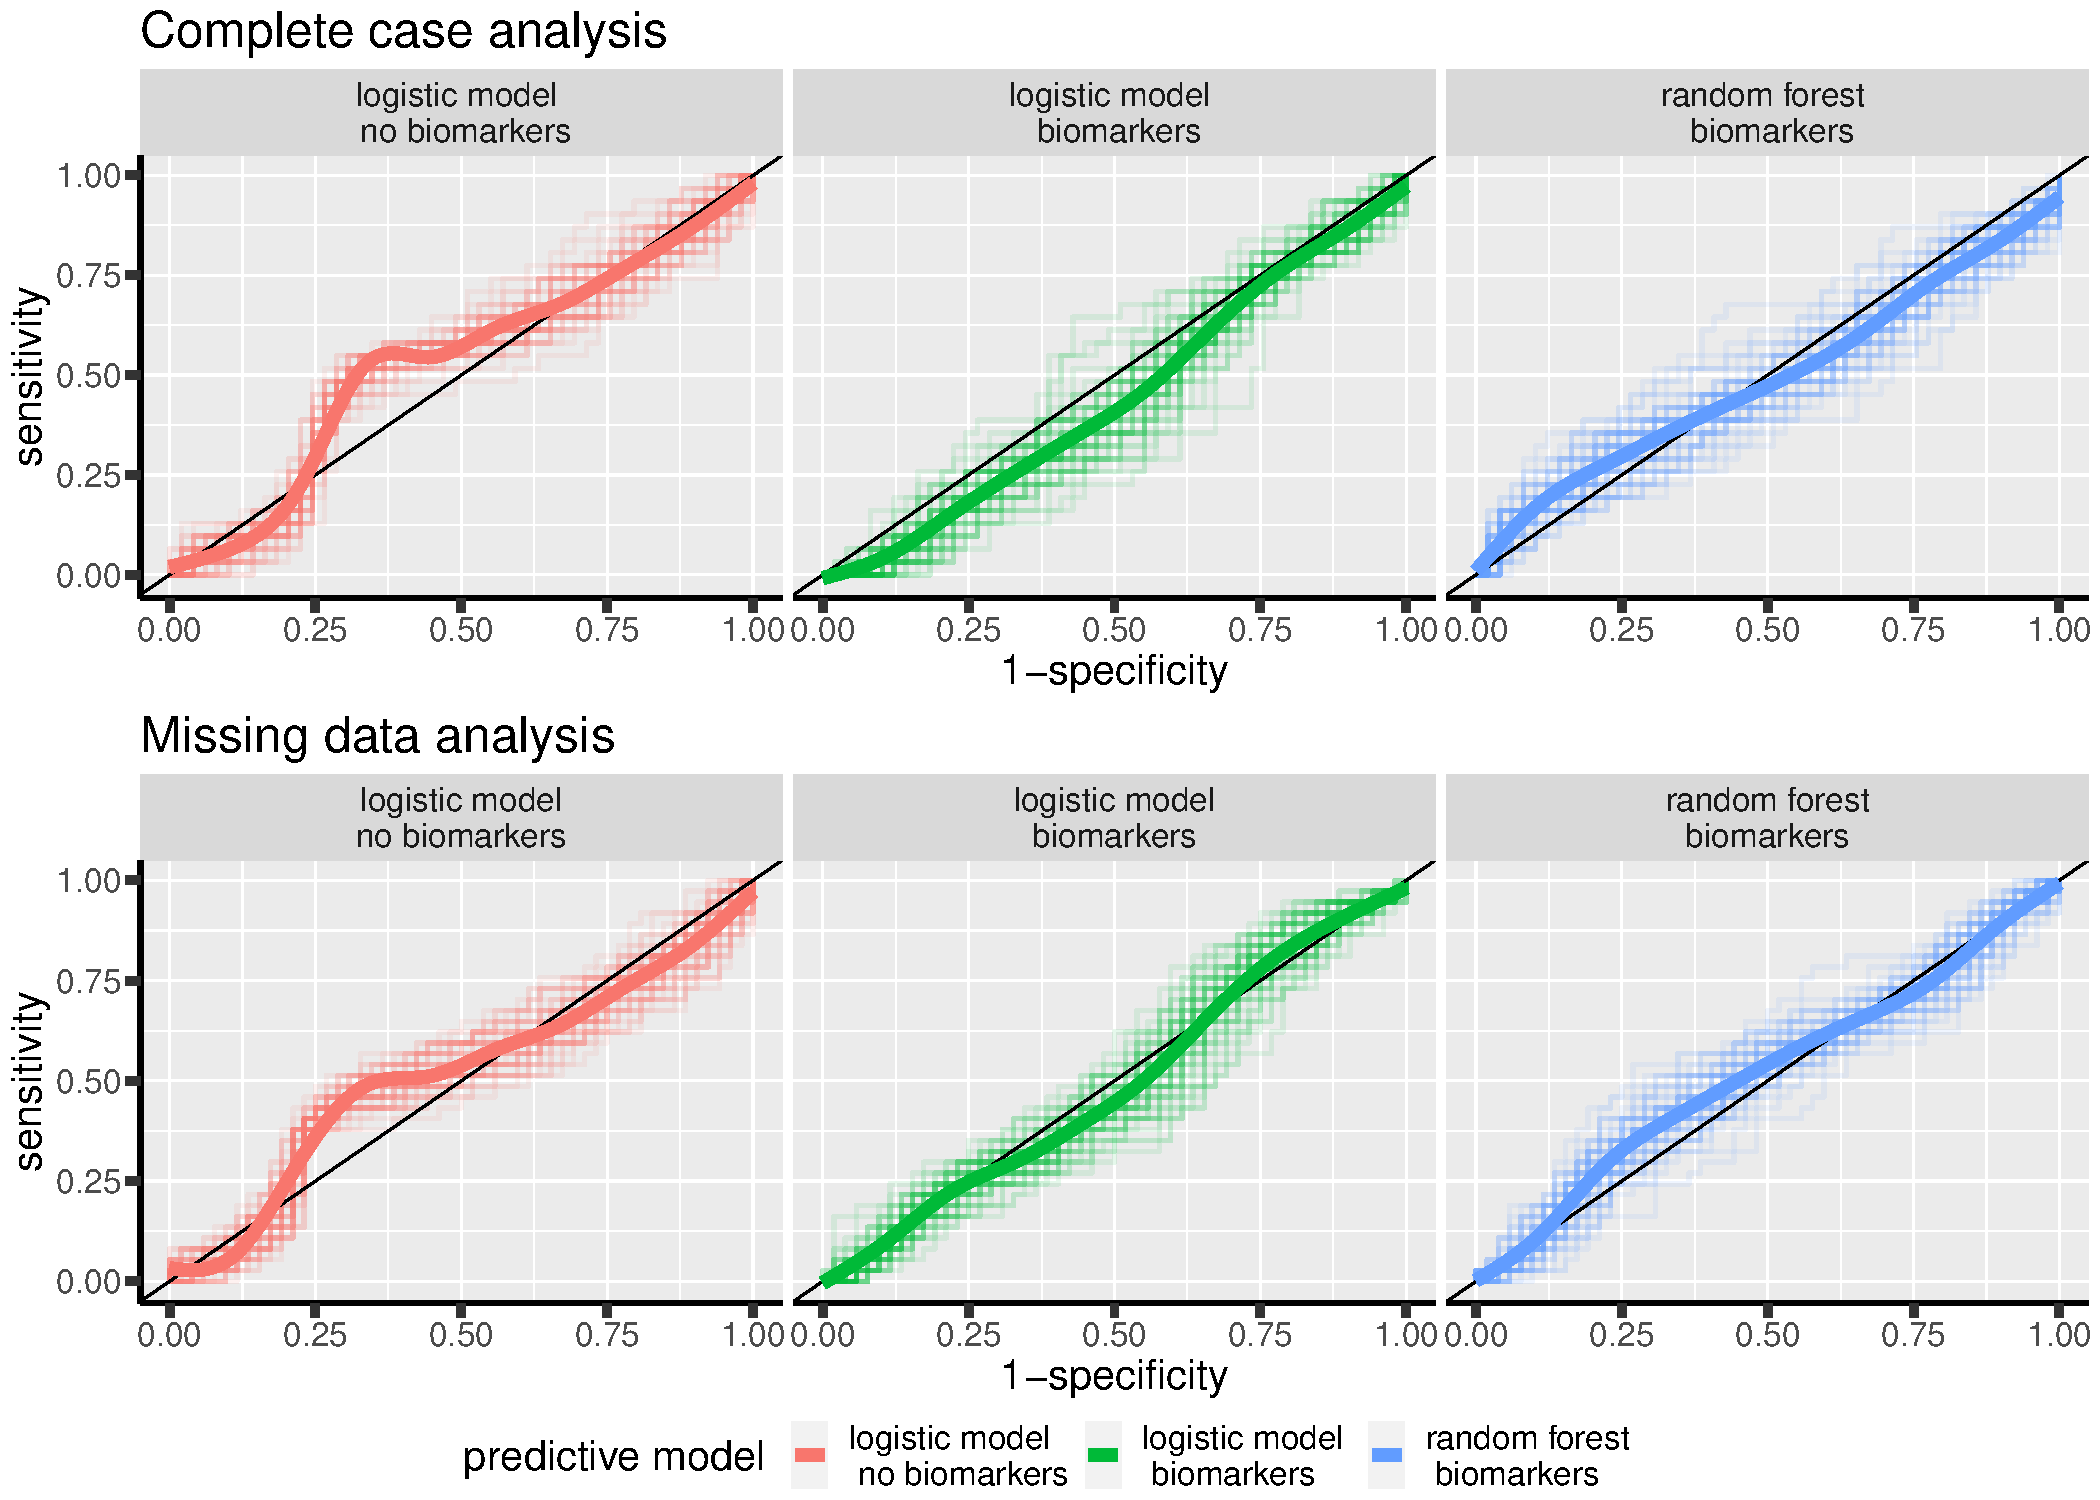
\includegraphics[trim={0 0 0 0},width=0.9\textwidth]{./../figures/ROC-pred-week4.pdf}
\caption{\label{fig:perfW4-ROC}Week 4}
\end{figure}

\begin{figure}[!h]
\centering
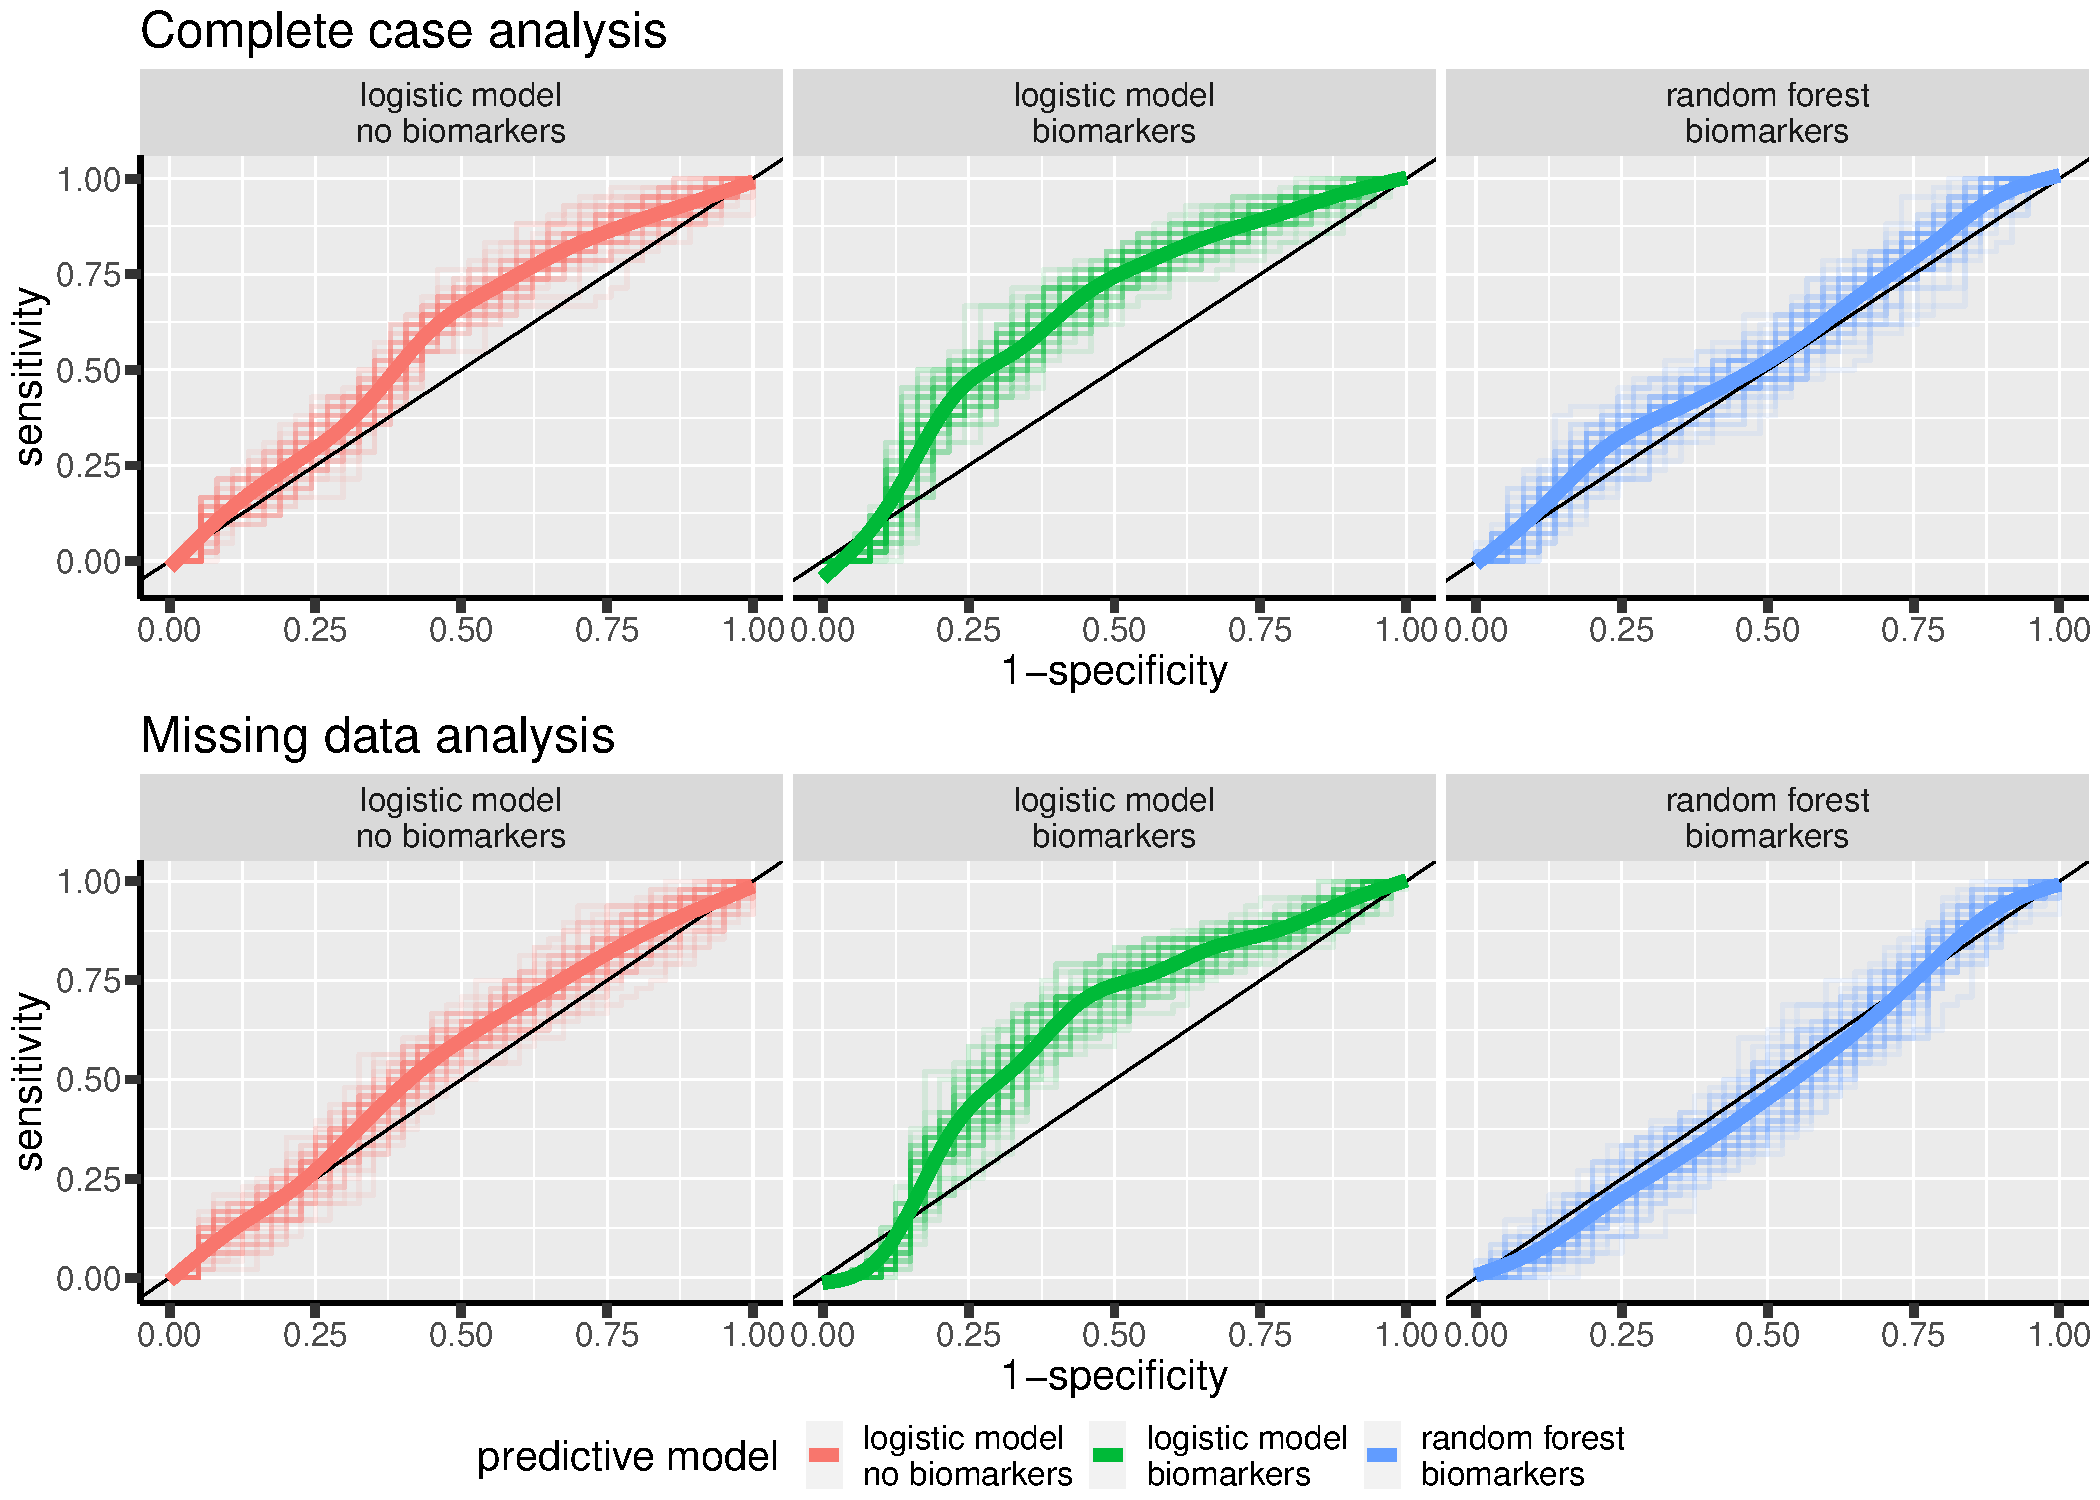
\includegraphics[trim={0 0 0 0},width=0.9\textwidth]{./../figures/ROC-pred-week8.pdf}
\caption{\label{fig:perfW8-ROC}Week 8}
\end{figure}

\begin{figure}[!h]
\centering
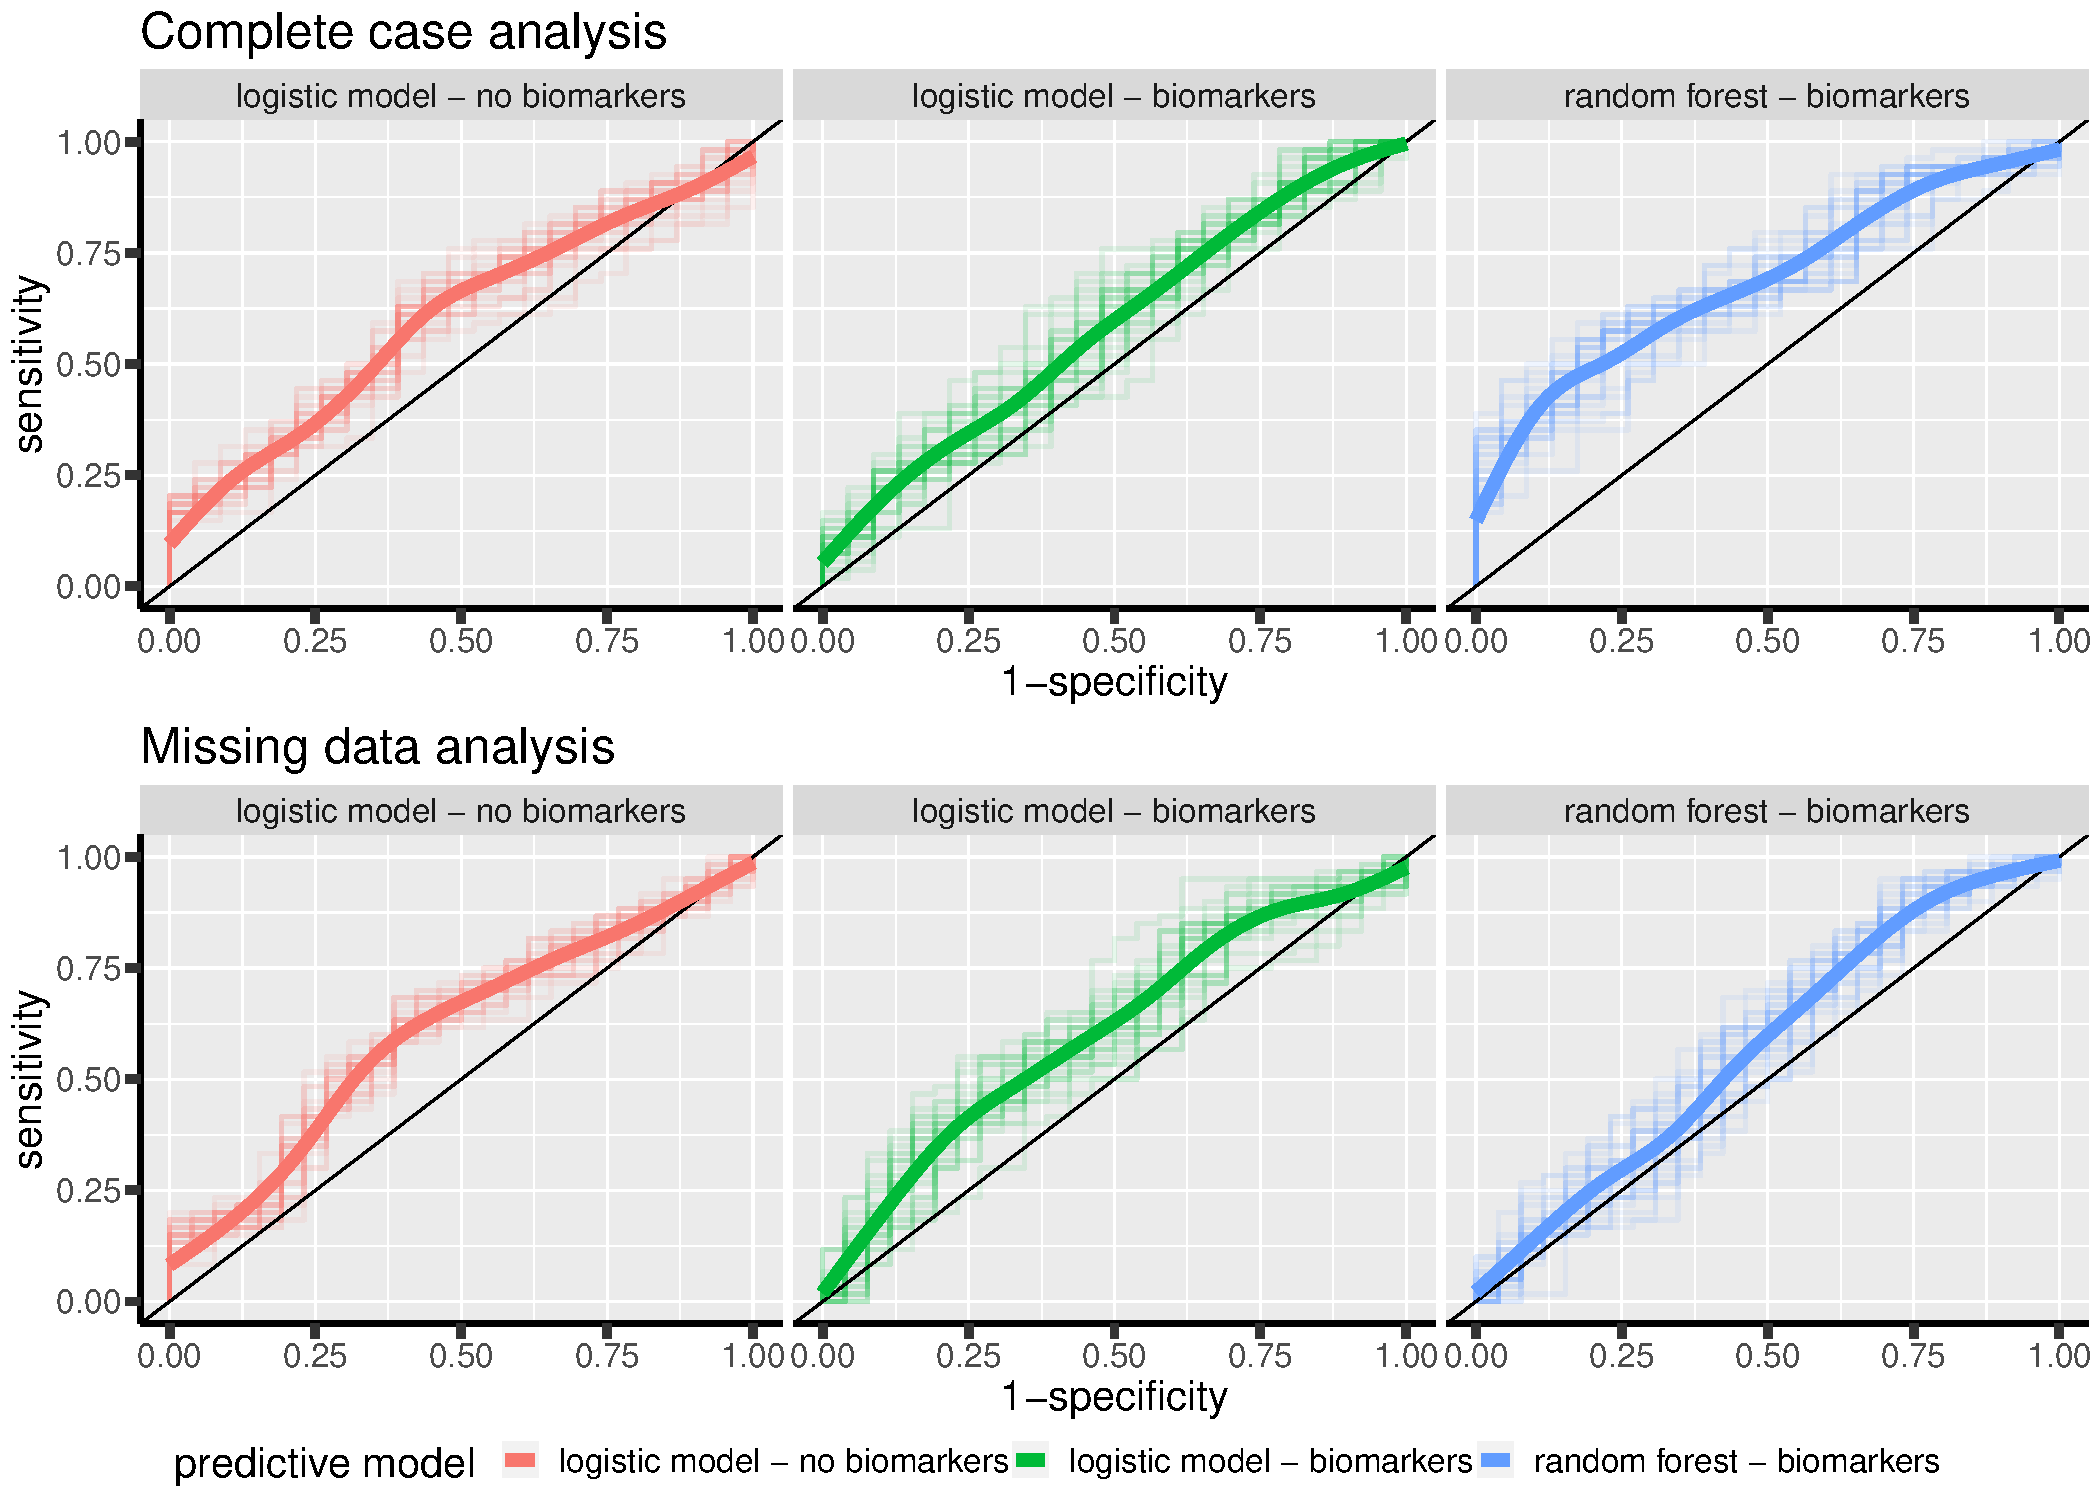
\includegraphics[trim={0 0 0 0},width=0.9\textwidth]{./../figures/ROC-pred-week12.pdf}
\caption{\label{fig:perfW12-ROC}Week 12}
\end{figure}


\clearpage
\section{Result for the secondary endpoint}
\label{appendix:trajectory}
\subsection{Association}
\label{sec:orgcb8b922}
Complete case analysis:
\phantomsection
\label{}
\begin{verbatim}
                     term    estimate    p.value adj.p.value  lower.adj upper.adj
 1:    MR (OFC thickness) -0.57903818 0.06505917   0.3643020 -1.4193293 0.2612529
 2:                HAMD17 -0.14949517 0.58610865   0.9975014 -0.8845609 0.5855706
 3:                 hsCRP  1.07690702 0.11793043   0.5687535 -0.7670841 2.9208981
 4:       PET (serotonin) -0.03633292 0.89032700   0.9999998 -0.7417565 0.6690907
 5: cognition (cluster 2) -0.46571118 0.45086576   0.9824984 -2.1193669 1.1879446
 6: cognition (cluster 3) -0.74402259 0.27045906   0.8791945 -2.5515550 1.0635098
 7:       EEG (vigilance) -0.56626760 0.06439629   0.3612880 -1.3859935 0.2534583
 8:                   age  0.27975595 0.29517902          NA         NA        NA
 9:                female -1.31928328 0.02054335          NA         NA        NA
10:                  CATS          NA         NA          NA         NA        NA
11:              Cortisol          NA         NA          NA         NA        NA
12:           Neuroticism          NA         NA          NA         NA        NA
\end{verbatim}

Missing data analysis:
\phantomsection
\label{}
\begin{verbatim}
                     term     estimate     p.value adj.p.value    lower.adj  upper.adj
 1:    MR (OFC thickness) -0.566732901 0.070380409   0.4817701 -1.452753857 0.31928806
 2:                HAMD17  0.025725243 0.929225742   1.0000000 -0.802720677 0.85417116
 3:                 hsCRP  1.253839863 0.079946120   0.5269300 -0.773390954 3.28107068
 4:       PET (serotonin)  0.048260858 0.848744807   1.0000000 -0.675460236 0.77198195
 5: cognition (cluster 2) -0.785645174 0.250978513   0.9230299 -2.733349473 1.16205912
 6: cognition (cluster 3) -1.039017852 0.130431392   0.7109416 -2.987458173 0.90942247
 7:       EEG (vigilance) -0.606743948 0.055133566   0.4019181 -1.500556688 0.28706879
 8:                  CATS -0.029002047 0.347080265   0.9778696 -0.116952688 0.05894859
 9:              Cortisol  0.003301743 0.293144971   0.9543628 -0.005644909 0.01224839
10:           Neuroticism -0.003265826 0.574591571   0.9996056 -0.019890752 0.01335910
11:                female -1.686694064 0.008284188          NA           NA         NA
12:                   age  0.276194477 0.318494902          NA           NA         NA
\end{verbatim}


\begin{figure}[!h]
\centering
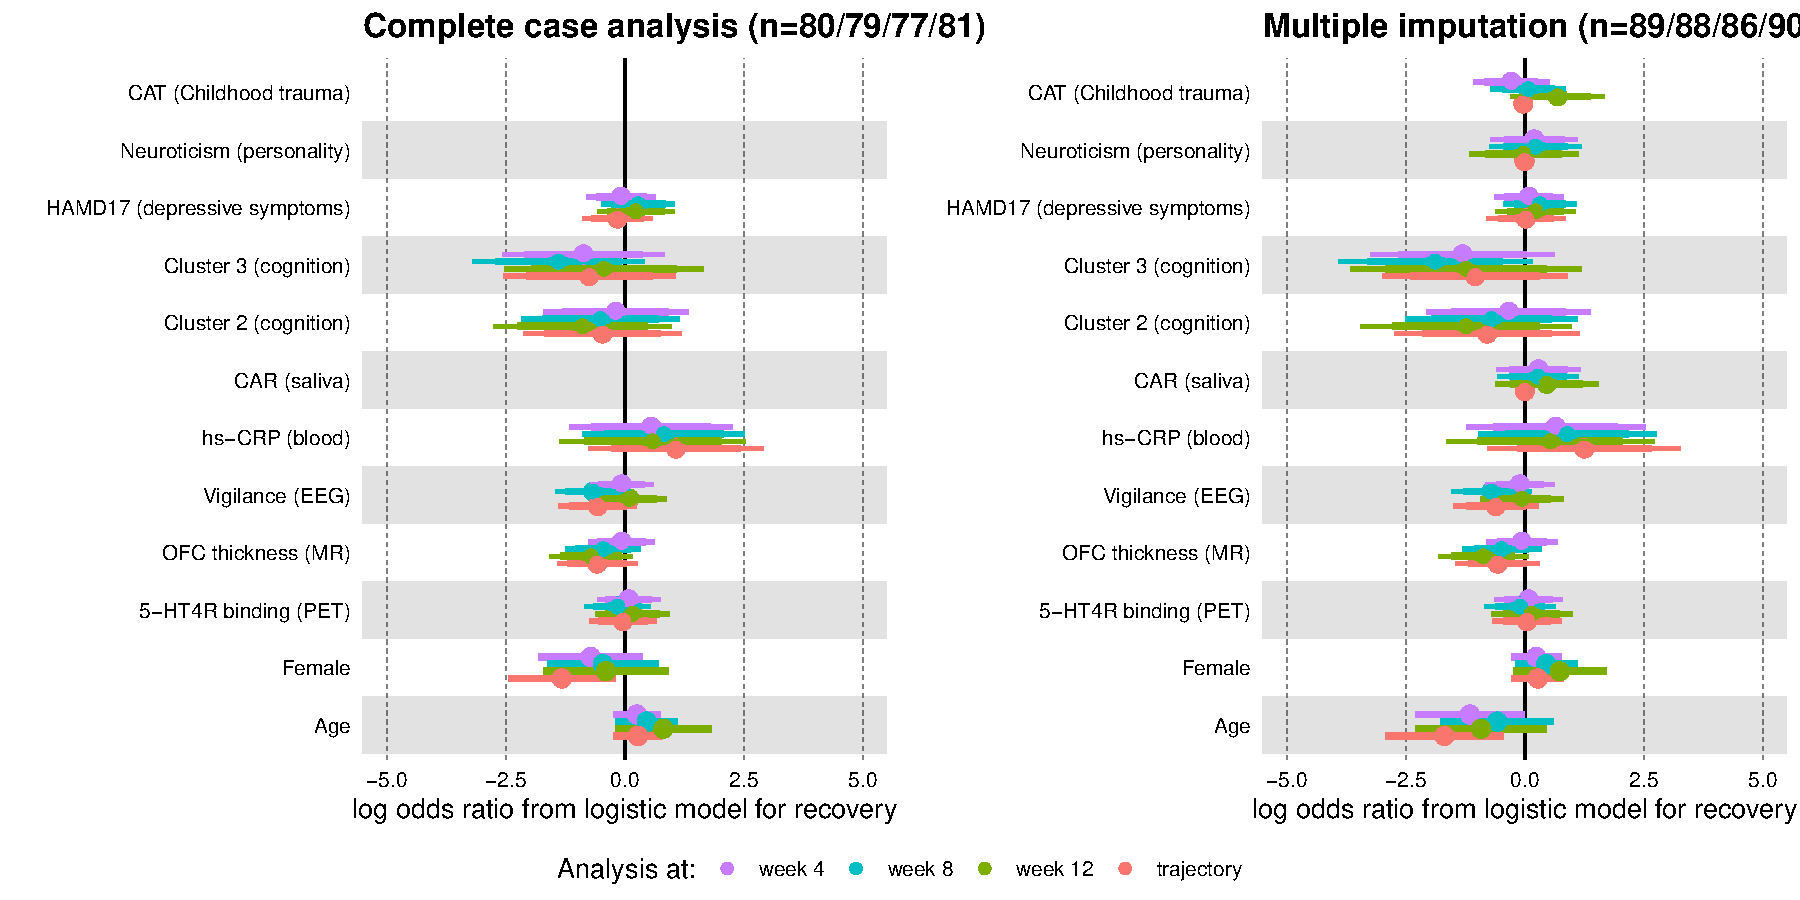
\includegraphics[trim={0 0 0 0},width=\textwidth]{./../figures/gg-forestplot-OR-traj.pdf}
\caption{Log-odd ratio estimates (full circles), confidence intervals (thick lines) and adjusted confidence intervals (thin lines) for each analysis at each timepoint. Covariates have been centered and scale to be comparable. Adjustment for multiplicity is performed over biomarkers but not over time.}
\end{figure}

\clearpage
\subsection{Prediction}
\label{sec:orgeb1046b}

\phantomsection
\label{}
\begin{verbatim}
                 model       week                                AUC                 Brier
 1: GLM (no biomarker)          4 0.514 (p(IF)=0.812, p(perm)=0.272) 0.245 (p(perm)=0.179)
 2:                             8 0.549 (p(IF)=0.420, p(perm)=0.152) 0.253 (p(perm)=0.289)
 3:                            12 0.622 (p(IF)=0.079, p(perm)=0.031) 0.204 (p(perm)=0.033)
 4:                    trajectory 0.586 (p(IF)=0.166, p(perm)=0.056) 0.231 (p(perm)=0.025)
 5:   GLM (biomarkers)          4 0.489 (p(IF)=0.847, p(perm)=0.521) 0.287 (p(perm)=0.471)
 6:                             8 0.621 (p(IF)=0.059, p(perm)=0.068) 0.258 (p(perm)=0.057)
 7:                            12 0.617 (p(IF)=0.098, p(perm)=0.072) 0.227 (p(perm)=0.061)
 8:                    trajectory 0.609 (p(IF)=0.080, p(perm)=0.048)  0.26 (p(perm)=0.068)
 9:    RF (biomarkers)          4  0.52 (p(IF)=0.739, p(perm)=0.390) 0.256 (p(perm)=0.399)
10:                             8 0.478 (p(IF)=0.710, p(perm)=0.596) 0.269 (p(perm)=0.615)
11:                            12 0.635 (p(IF)=0.044, p(perm)=0.044) 0.203 (p(perm)=0.050)
12:                    trajectory 0.546 (p(IF)=0.444, p(perm)=0.257) 0.247 (p(perm)=0.252)
\end{verbatim}
\end{document}
